\documentclass[a4paper]{article}
\usepackage{inputenc}
\usepackage[british,UKenglish]{babel}
\usepackage{amsmath}
%\usepackage{titlesec}
\usepackage{color}
\usepackage{graphicx}
\usepackage{fancyref}
\usepackage{hyperref}
\usepackage{float}
\usepackage{scrextend}
\usepackage{setspace}
\usepackage{xargs}
\usepackage{multicol}
\usepackage{nameref}

\usepackage{sectsty}
\usepackage{multicol}
\usepackage{multirow}
\usepackage[procnames]{listings}
\usepackage{appendix}

\newcommand\tab[1][1cm]{\hspace*{#1}}
\hypersetup{colorlinks=true, linkcolor=black}
\interfootnotelinepenalty=10000

\newcommand{\cleancode}[1]{\begin{addmargin}[3em]{3em}\texttt{\textcolor{cleanOrange}{#1}}\end{addmargin}}
\newcommand{\cleanstyle}[1]{\text{\textcolor{cleanOrange}{\texttt{#1}}}}


\usepackage[colorinlistoftodos,prependcaption,textsize=footnotesize]{todonotes}
\newcommandx{\commred}[2][1=]{\textcolor{Red}
{\todo[linecolor=red,backgroundcolor=red!25,bordercolor=red,#1]{#2}}}
\newcommandx{\commblue}[2][1=]{\textcolor{Blue}
{\todo[linecolor=blue,backgroundcolor=blue!25,bordercolor=blue,#1]{#2}}}
\newcommandx{\commgreen}[2][1=]{\textcolor{OliveGreen}{\todo[linecolor=OliveGreen,backgroundcolor=OliveGreen!25,bordercolor=OliveGreen,#1]{#2}}}
\newcommandx{\commpurp}[2][1=]{\textcolor{Plum}{\todo[linecolor=Plum,backgroundcolor=Plum!25,bordercolor=Plum,#1]{#2}}}

\def\code#1{{\tt #1}}

\def\note#1{\noindent{\bf [Note: #1]}}

\makeatletter
%% The "\@seccntformat" command is an auxiliary command
%% (see pp. 26f. of 'The LaTeX Companion,' 2nd. ed.)
\def\@seccntformat#1{\@ifundefined{#1@cntformat}%
   {\csname the#1\endcsname\quad}  % default
   {\csname #1@cntformat\endcsname}% enable individual control
}
\let\oldappendix\appendix %% save current definition of \appendix
\renewcommand\appendix{%
    \oldappendix
    \newcommand{\section@cntformat}{\appendixname~\thesection\quad}
}
\makeatother


% "define" Scala
\usepackage[T1]{fontenc}  
\usepackage[scaled=0.82]{beramono}  
\usepackage{microtype} 

\sbox0{\small\ttfamily A}
\edef\mybasewidth{\the\wd0 }

\lstdefinelanguage{scala}{
  morekeywords={abstract,case,catch,class,def,%
    do,else,extends,false,final,finally,%
    for,if,implicit,import,match,mixin,%
    new,null,object,override,package,%
    private,protected,requires,return,sealed,%
    super,this,throw,trait,true,try,%
    type,val,var,while,with,yield},
  sensitive=true,
  morecomment=[l]{//},
  morecomment=[n]{/*}{*/},
  morestring=[b]",
  morestring=[b]',
  morestring=[b]"""
}

\usepackage{color}
\definecolor{dkgreen}{rgb}{0,0.6,0}
\definecolor{gray}{rgb}{0.5,0.5,0.5}
\definecolor{mauve}{rgb}{0.58,0,0.82}

% Default settings for code listings
\lstset{frame=tb,
  language=scala,
  aboveskip=3mm,
  belowskip=3mm,
  showstringspaces=false,
  columns=fixed, % basewidth=\mybasewidth,
  basicstyle={\small\ttfamily},
  numbers=none,
  numberstyle=\footnotesize\color{gray},
  % identifierstyle=\color{red},
  keywordstyle=\color{blue},
  commentstyle=\color{dkgreen},
  stringstyle=\color{mauve},
  frame=single,
  breaklines=true,
  breakatwhitespace=true,
  procnamekeys={def, val, var, class, trait, object, extends},
  procnamestyle=\ttfamily\color{red},
  tabsize=2
}

\lstnewenvironment{scala}[1][]
{\lstset{language=scala,#1}}
{}
\lstnewenvironment{cpp}[1][]
{\lstset{language=C++,#1}}
{}
\lstnewenvironment{bash}[1][]
{\lstset{language=bash,#1}}
{}
\lstnewenvironment{verilog}[1][]
{\lstset{language=verilog,#1}}
{}



\graphicspath{ {images/} }
\usepackage{ctex}
\usepackage{graphicx}
\usepackage{color,framed}%文本框
\usepackage{listings}
\usepackage{caption}

\usepackage{hyperref}
\hypersetup{hidelinks,
	colorlinks=true,
	allcolors=black,
	pdfstartview=Fit,
	breaklinks=true}


\lstdefinestyle{mystyle}{
  keywordstyle=\color{orange},  % 设置关键词颜色为橙色
 morekeywords={set, nmap, msfconsole,exploit},           % 仅将 set 设置为橙色
}

\usepackage{amssymb}
\usepackage{enumerate}
\usepackage{xcolor}
\usepackage{bm} 
\usepackage{lastpage}%获得总页数
\usepackage{fancyhdr}
\usepackage{tabularx}  
\usepackage{geometry}
\usepackage{minted}
\usepackage{graphics}
\usepackage{subfigure}
\usepackage{float}
\usepackage{pdfpages}
\usepackage{pgfplots}
\pgfplotsset{width=10cm,compat=1.9}
\usepackage{multirow}
\usepackage{footnote}
\usepackage{booktabs}
\usepackage{listings}

%-----------------------伪代码------------------
\usepackage{algorithm}  
\usepackage{algorithmicx}  
\usepackage{algpseudocode}  
\floatname{algorithm}{Algorithm}  
\renewcommand{\algorithmicrequire}{\textbf{Input:}}  
\renewcommand{\algorithmicensure}{\textbf{Output:}} 
\usepackage{lipsum}  
\makeatletter
\newenvironment{breakablealgorithm}
  {% \begin{breakablealgorithm}
  \begin{center}
     \refstepcounter{algorithm}% New algorithm
     \hrule height.8pt depth0pt \kern2pt% \@fs@pre for \@fs@ruled
     \renewcommand{\caption}[2][\relax]{% Make a new \caption
      {\raggedright\textbf{\ALG@name~\thealgorithm} ##2\par}%
      \ifx\relax##1\relax % #1 is \relax
         \addcontentsline{loa}{algorithm}{\protect\numberline{\thealgorithm}##2}%
      \else % #1 is not \relax
         \addcontentsline{loa}{algorithm}{\protect\numberline{\thealgorithm}##1}%
      \fi
      \kern2pt\hrule\kern2pt
     }
  }{% \end{breakablealgorithm}
     \kern2pt\hrule\relax% \@fs@post for \@fs@ruled
  \end{center}
  }
\makeatother
%------------------------代码-------------------
\RequirePackage{listings}
\RequirePackage{xcolor}
\definecolor{dkgreen}{rgb}{0,0.6,0}
\definecolor{gray}{rgb}{0.5,0.5,0.5}
\definecolor{mauve}{rgb}{0.58,0,0.82}
\lstset{
	numbers=left,  
	frame=tb,
	aboveskip=3mm,
	belowskip=3mm,
	showstringspaces=false,
	columns=flexible,
	framerule=1pt,
	rulecolor=\color{gray!35},
	backgroundcolor=\color{gray!5},
	basicstyle={\ttfamily},
	numberstyle=\tiny\color{gray},
	keywordstyle=\color{blue},
	commentstyle=\color{dkgreen},
	stringstyle=\color{mauve},
	breaklines=true,
	breakatwhitespace=true,
	tabsize=3,
}


%-------------------------页面边距--------------
\geometry{a4paper,left=2.5cm,right=2.5cm,top=2.6cm,bottom=2.7cm}
%-------------------------页眉页脚--------------
\usepackage{fancyhdr}
\pagestyle{fancy}
\lhead{\kaishu }
\chead{}
\rhead{{\CJKfontspec{simkai.ttf} }}
\lfoot{}
\cfoot{\thepage}
\rfoot{}
\renewcommand{\headrulewidth}{0pt}  
\renewcommand{\footrulewidth}{0pt}
\newcommand{\HRule}{\rule{\linewidth}{0.5mm}}
\newcommand{\HRulegrossa}{\rule{\linewidth}{1.2mm}}
\setlength{\textfloatsep}{10mm}
%--------------------文档内容--------------------
\renewcommand{\contentsname}{目\ 录}
\renewcommand{\appendixname}{附录}
\renewcommand{\appendixpagename}{附录}
\renewcommand{\refname}{参考文献} 
\renewcommand{\figurename}{图}
\renewcommand{\tablename}{表}
\renewcommand{\today}{\number\year 年 \number\month 月 \number\day 日}

\renewcommand {\thefigure}{\thesection{}.\arabic{figure}}%图片按章标号
\renewcommand{\figurename}{图}
\renewcommand{\contentsname}{目录}  
\cfoot{\thepage\ of \pageref{LastPage}}%当前页 of 总页数

\renewcommand{\abstractname}{\textbf{\Large 摘要}} % 调整摘要标题的字体大小
\renewcommand {\thefigure}{\thesection{}.\arabic{figure}}%图片按章标号

\begin{document}

\renewcommand{\figurename}{图}
\renewcommand{\contentsname}{目录}  
\cfoot{\thepage\ of \pageref{LastPage}}
\renewcommand{\abstractname}{\textbf{\Large 摘要}} 

\begin{center}
    \huge{\textbf{体系结构第一次实验报告}}
\end{center}

\begin{center}
    \textbf{姓名}:\underline{梁朝阳} \quad
    \textbf{专业}:\underline{密码科学与技术}
\end{center}

\tableofcontents

\vspace*{1cm}

\noindent{\Large\textbf{摘要}}

\vspace{1em}

\textbf{CPU结构部分:} 我打算从相关性的级联控制开始谈我的理解,之后CPU最复杂的地方莫过于控制信号的设计,这部分内容我需要阅读decode.v文件来理解。还有就是我会讲下我对CP0寄存器的理解。最后我会说下我对延迟槽机制实现的理解,并做出我认为当前CPU的运行没有错误的判断。(当然IP核的配置不是按上学期照操作手册上描述的那样,需要取消Primitive register的使用)。

\textbf{新增指令部分:} 我会逐一介绍新增的9条指令,大多数都是关于CP0寄存器的操作。还有一部分是乘法器指令有关的指令。

\vspace{1em}
\noindent\textbf{关键词:} 流水线CPU,CP0寄存器,延迟槽,乘法器
\newpage


\section{实验目的}

\begin{enumerate}
    \item 熟悉并掌握流水线 CPU 的原理和设计。
    \item 检验运用 verilog 语言进行电路设计的能力。
    \item 通过亲自设计实现静态 5 级流水线 CPU,加深对计算机组成原理和体系结构理
    论知识的理解。
\end{enumerate}

\section{实验要求}

\begin{enumerate}
    \item 修改原始代码source code中的bug,保证指令运行正确
    \item 针对五级流水线中新增加的指令,逐级分析指令执行过程和执行结果,梳理流水线知识点
\end{enumerate}

\section{实验过程}

\subsection{熟悉代码|CPU结构部分}

\subsubsection{相关性的级联控制}

最重要的肯定是级联控制,与理论课上从相关性检测单元来控制的方法不同,这里的级联控制是基于两个阶段的握手信号来实现的:

\begin{figure}[H]
    \centering
    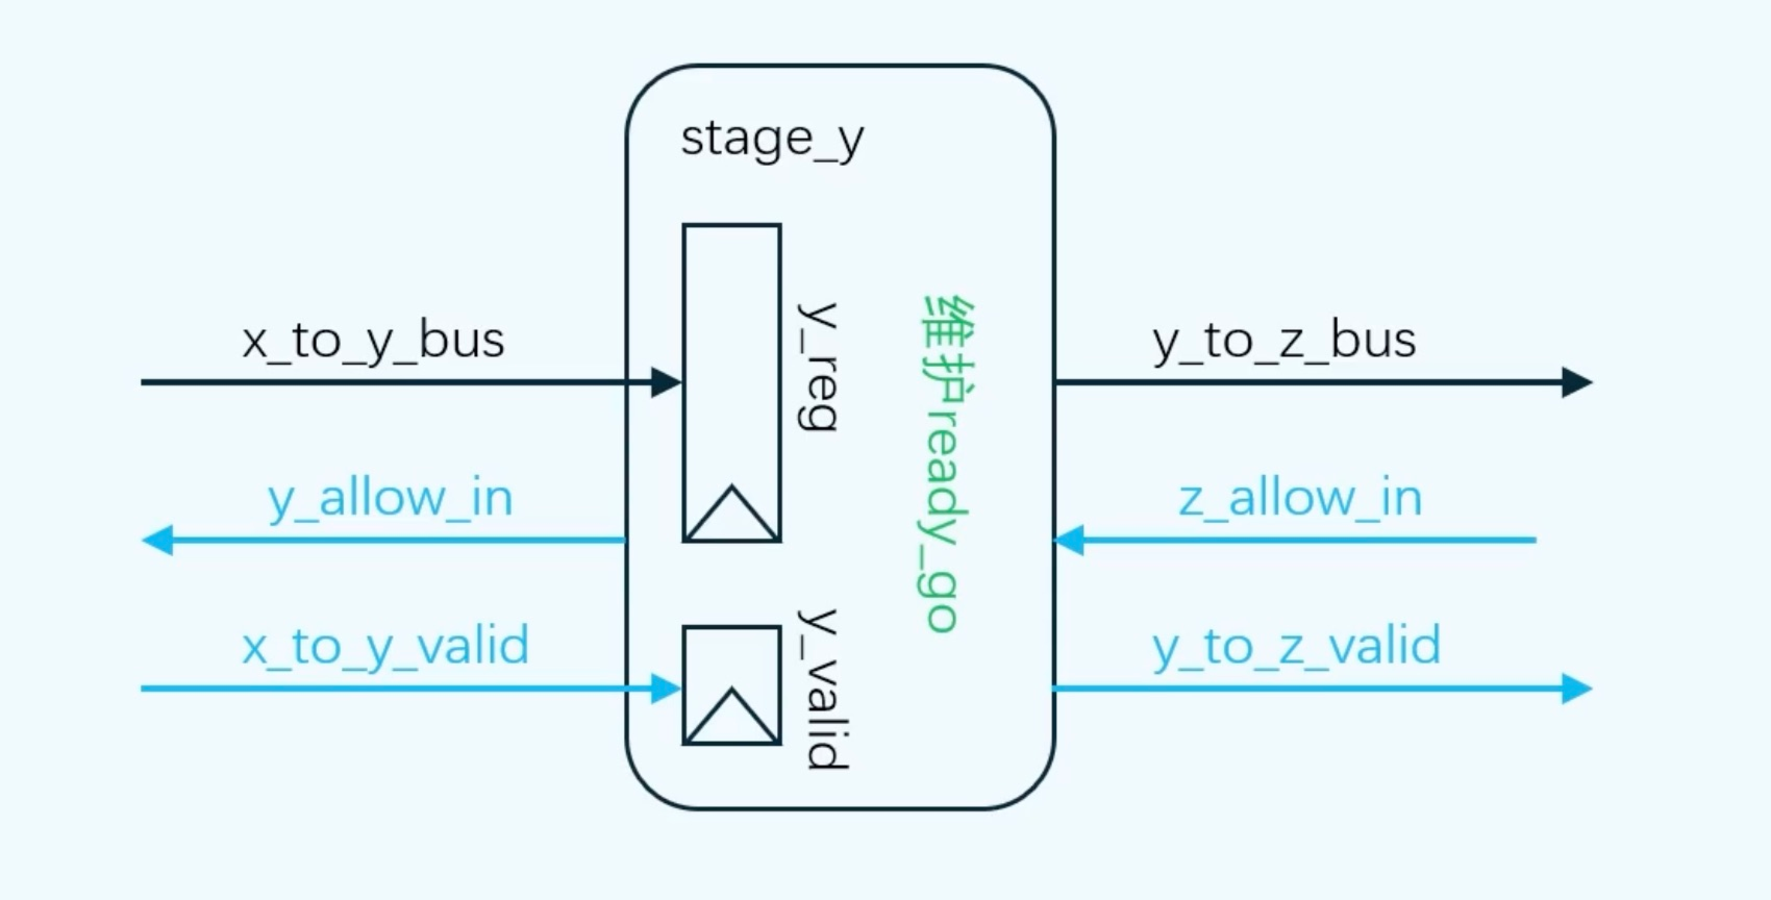
\includegraphics[width=0.8\textwidth]{img/复现流水线/级联控制.pdf}
    \caption{相关性的级联控制}
\end{figure}

以最一般的stage\_y举例,这里一共有这7个信号:
\begin{enumerate}
    \item \texttt{x\_to\_y\_bus} :x阶段到y阶段的总线
    \item \texttt{y\_allow\_in} :(本实验代码中实现为 \texttt{y\_over} 信号)y阶段允许x阶段的数据进入
    \item \texttt{x\_to\_y\_valid} :x阶段到y阶段的数据有效(即\texttt{x\_to\_y\_bus} 有效)
    \item \texttt{y\_to\_z\_bus} :y阶段到z阶段的总线
    \item \texttt{z\_allow\_in} :(本实验代码中实现为 \texttt{z\_over} 信号)z阶段允许y阶段的数据进入
    \item \texttt{y\_to\_z\_valid}:y阶段到z阶段的数据有效(即\texttt{y\_to\_z\_bus} 有效)
    \item \texttt{ready\_go}:是否为1取决于y阶段是否完成,这个在每个阶段的具体实现不同,例如本实验在乘法器的地方叫做\texttt{mult\_end},在存储的时候比较复杂,没有给出显式的ready\_go信号,而是给出了下面这个代码,这里的\texttt{inst\_load ? MEM\_valid\_r : MEM\_valid}实际上就是ready\_go信号,从其能够影响(控制)over信号可以看出,其中over本质上就是to\_next\_stage信号.
    \begin{lstlisting}[language=Verilog]
        assign MEM_over = inst_load ? MEM_valid_r : MEM_valid;
    \end{lstlisting}    
\end{enumerate}
以及如下两个寄存器:
\begin{enumerate}
    \item \texttt{y\_reg} :y阶段的数据寄存器,用于接受\texttt{x\_to\_y\_bus}的数据
    \item \texttt{y\_valid}:这个信号比较重要,具体地:
    \begin{enumerate}
        \item x 阶段的数据有效且 y 阶段 可以接收数据,则为1
        \item x 阶段数据无效且 y 阶段 可以接收数据,则为0 (这里要注意,有些运算并不能够一周期完成,因此如果y不可接受数据,那么\_valid 应当保持不变)
        \item rest或者cancel的时候为0
    \end{enumerate}
    那么我总结一下这个信号本身意思是标记当前阶段数据是否有效,为1的情况有两种,一种是当前数据有效正在进行多周期运算/被阻塞,另一种是当前数据有效且下一个周期就要走了,这个时候allow\_in也为1,那么下一个周期仍然是有效的(需要赋值为1)。
\end{enumerate}

具体地,这个信号这么实现:

\begin{figure}[H]
    \centering
    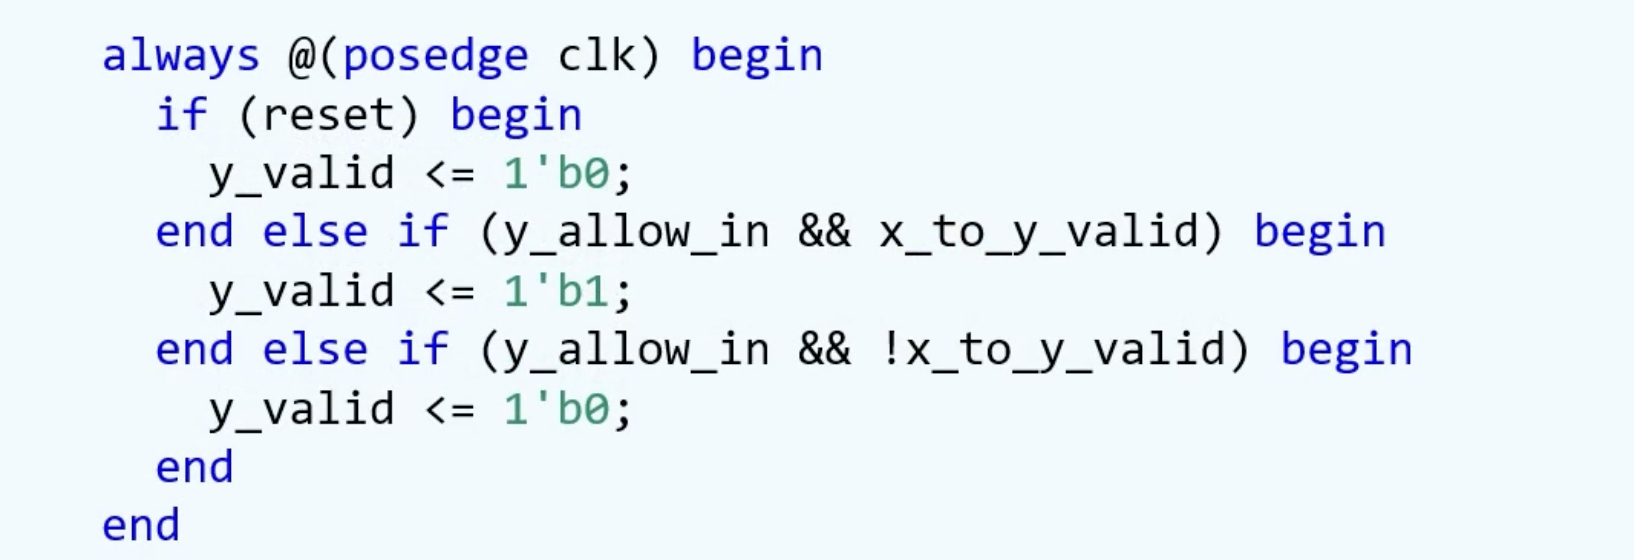
\includegraphics[width=0.8\textwidth]{img/复现流水线/级联控制valid信号.png}
    \caption{级联控制valid信号}
    \label{fig:级联控制valid信号}
\end{figure}

其中可以简化实现为将y\_valid直接赋值为x\_to\_y\_valid,当y\_allow\_in为1的时候。

其余的信号也简单说下是怎么实现的,这里直接给出实验中的CPU的代码,我们这里统一使用EXE阶段的信号举例:

\paragraph{EXE\_valid}这里说下实验中是如何实现valid信号的,以EXE\_valid为例:

\begin{lstlisting}[language=Verilog]
    //EXE_valid
    always @(posedge clk)
    begin
        if (!resetn || cancel)
        begin
            EXE_valid <= 1'b0;
        end
        else if (EXE_allow_in)
        begin
            EXE_valid <= ID_over;
        end
    end
\end{lstlisting}

这里是ID对EXE实现握手,ID\_over就是ID\_allow\_in。这里的行为完全符合我刚才对图\ref{fig:级联控制valid信号}的分析。

\paragraph{EXE\_allow\_in}

还有allow\_in信号,这个信号用于告诉前一个阶段自己是否可以接收数据:

\begin{lstlisting}[language=Verilog]
    assign EXE_allow_in = ~EXE_valid | (EXE_over & MEM_allow_in);
\end{lstlisting}

可以看到,当本阶段没有有效数据(为空)的时候肯定是可以接受数据的。或者下一个阶段我这个阶段的数据就要走了,那么也可以接受。反之stall。

\paragraph{锁存(总线传输)}

当我这个阶段结束,且下一个阶段允许我流出的时候,我就可以把上一个给我的信号存到reg寄存器中。注意,这里我们采用的是永远让后一个stage维护reg的实现方式。

\begin{lstlisting}[language=Verilog]
    always @(posedge clk)
    begin
        if(EXE_over && MEM_allow_in)
        begin
            EXE_MEM_bus_r <= EXE_MEM_bus;
        end
    end
\end{lstlisting}


到这里我认为级联控制部分就介绍完了。

\subsubsection{decoder 的控制信号的设计}

控制信号设计较为困难,我们分成多个小模块讲解:

\paragraph{解码} 解码操作是将指令分解为各个部分,例如操作码、源操作数、目标操作数等。

\begin{lstlisting}[language=Verilog]
    assign op     = inst[31:26];  // 操作码
    assign rs     = inst[25:21];  // 源操作数1
    ... \\ 手动省略几个,水字数没意义,就是把32位地址拆开了
    assign target = inst[25:0];   // 目标地址
    assign cp0r_sel= inst[2:0];   // cp0寄存器的select域
\end{lstlisting}

这里是解码器的一部分,用于把inst 分解为各个部分。

接着是一对的assign语句,把满足某个指令条件的信号赋值为1,举一个最简单的例子:

\begin{lstlisting}[language=Verilog]
    assign inst_MULT  = op_zero & (rd==5'd0) & sa_zero & (funct == 6'b011000);             //乘法
\end{lstlisting}

这个的意思是:当操作码为0,特殊域为0,功能码为011000的时候,inst\_MULT为1。


\paragraph{ALU的控制信号}
接着是对ALU专门的信号控制,采用的是独热编码:

\begin{lstlisting}[language=Verilog]    
    assign alu_control = {inst_add,         
    inst_sub,
    inst_slt,
    inst_sltu,
    ... \\ 这里我手动省略几个,总之就是打包成一个总线给ALU
    inst_srl,
    inst_sra,
    inst_lui};
\end{lstlisting}

还有一个是ALU的两个操作数:

\begin{lstlisting}[language=Verilog]
    assign alu_operand1 = inst_j_link ? pc : 
                          inst_shf_sa ? {27'd0,sa} : rs_value;
    assign alu_operand2 = inst_j_link ? 32'd8 :  
                          inst_imm_zero ? {16'd0, imm} :
                          inst_imm_sign ?  {{16{imm[15]}}, imm} : rt_value;
\end{lstlisting}    

这里为什么说一下,是因为实现旁路的时候这里的后面是需要动一下的。例如加两个MUX:

\begin{figure}[H]
    \centering
    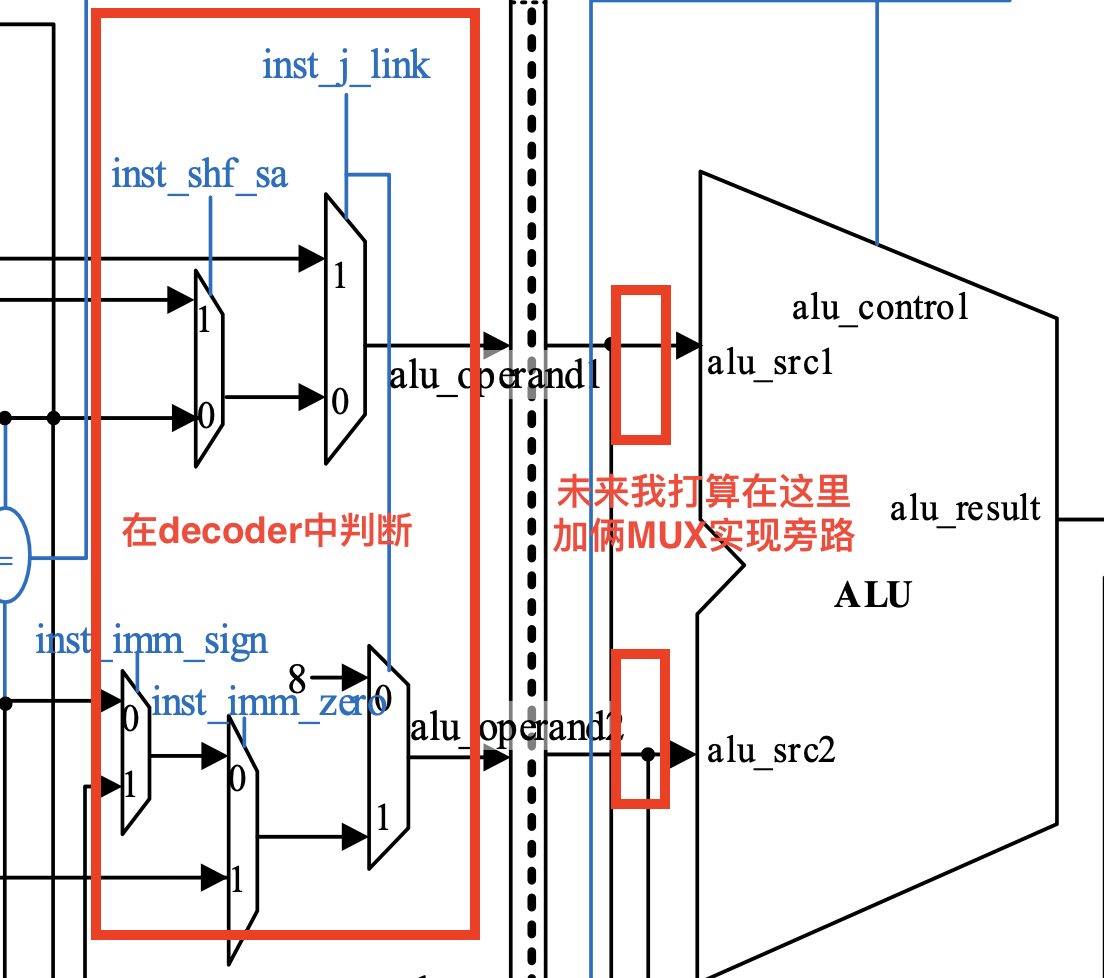
\includegraphics[width=0.65\textwidth]{img/复现流水线/ALU操作数.png}
    \caption{ALU操作数}
    \label{fig:ALU操作数}
\end{figure}

\subsubsection{CP0寄存器的理解(顺带HI和LO寄存器)}

到了CP0寄存器,这个CPO是Coprocessor 0的缩写,表示协处理器0。这个协处理器0是MIPS体系结构中的一个协处理器,用于实现一些特殊的功能,例如异常处理、中断处理等。

而HI和LO寄存器是用于存放乘法结果的,我打算单独一个地方说乘法的走线。而且在我的浅薄认知来看,一旦涉及这种某一个阶段可以跑多个周期,还是级联控制要简单很多。


\paragraph{WB阶段的控制信号}


要分析协处理器,就要看WB阶段:

\begin{lstlisting}[language=Verilog]
module wb(                       // 写回级
    input          WB_valid,     // 写回级有效
    input  [117:0] MEM_WB_bus_r, // MEM->WB总线
    output         rf_wen,       // 寄存器写使能
    output [  4:0] rf_wdest,     // 寄存器写地址
    output [ 31:0] rf_wdata,     // 寄存器写数据
    output         WB_over,      // WB模块执行完成

    // 省略常规信号如clk、resetn等
     output [ 32:0] exc_bus,      // Exception pc总线
     output [  4:0] WB_wdest,     // WB级要写回寄存器堆的目标地址号
     output         cancel,       // syscall和eret到达写回级时会发出cancel信号,取消已经取出的正在其他流水级执行的指令
    //省略展示信号
);
\end{lstlisting}

上述代码片段中,主要涉及写回阶段寄存器堆相关的输出信号说明如下:

\begin{enumerate}
    \item \texttt{rf\_wen}:写回阶段寄存器堆写使能信号,高电平时表示允许写寄存器。
    \item \texttt{rf\_wdest}:写回阶段寄存器堆写地址,指定要写入的目标寄存器编号。
    \item \texttt{rf\_wdata}:写回阶段写入寄存器堆的数据。
\end{enumerate}

这些信号共同完成了指令执行结果向寄存器堆的写回操作,是WB(写回)阶段的核心输出。

\paragraph{CP0寄存器的控制信号}

由于目前设计的CPU并不完备,所用到的cp0寄存器也很少,故暂时只实现STATUS(12.0),CAUSE(13.0),EPC(14.0)这三个。

其中mtc0 (move to coprocessor 0)和mfc0 (move from coprocessor 0)是用于向CP0寄存器写入和读取数据,mfhi (move from hi)和mflo (move from lo)是用于从HI和LO寄存器读取数据。

\begin{lstlisting}[language=Verilog]
    assign status_wen = mtc0 & (cp0r_addr=={5'd12,3'd0});
    assign epc_wen    = mtc0 & (cp0r_addr=={5'd14,3'd0});
\end{lstlisting}

其中5'd12,3'd0的含义是:5'd12表示STATUS寄存器,3'd0表示STATUS寄存器的第0位。 这里的编号(地址)是自己设计的。

\paragraph{CP0寄存器读取} 寄存器读取实现就是一个MUX,根据地址选择读取哪个寄存器。说实话,我并不是很喜欢这种嵌套的实现,感觉不如一个大寄存器清晰,但是我猜测可能这样实现起来映射到硬件上更简单,毕竟这个是一堆的两个入口的MUX。

\begin{lstlisting}[language=Verilog]
    assign cp0r_rdata = (cp0r_addr=={5'd12,3'd0}) ? cp0r_status :
                       (cp0r_addr=={5'd13,3'd0}) ? cp0r_cause  :
                       (cp0r_addr=={5'd14,3'd0}) ? cp0r_epc : 32'd0;
\end{lstlisting}

但是,设计图中画的是一个大的MUX,而代码是先判断两个,然后接着判断后面的:

\begin{figure}[H]
    \centering
    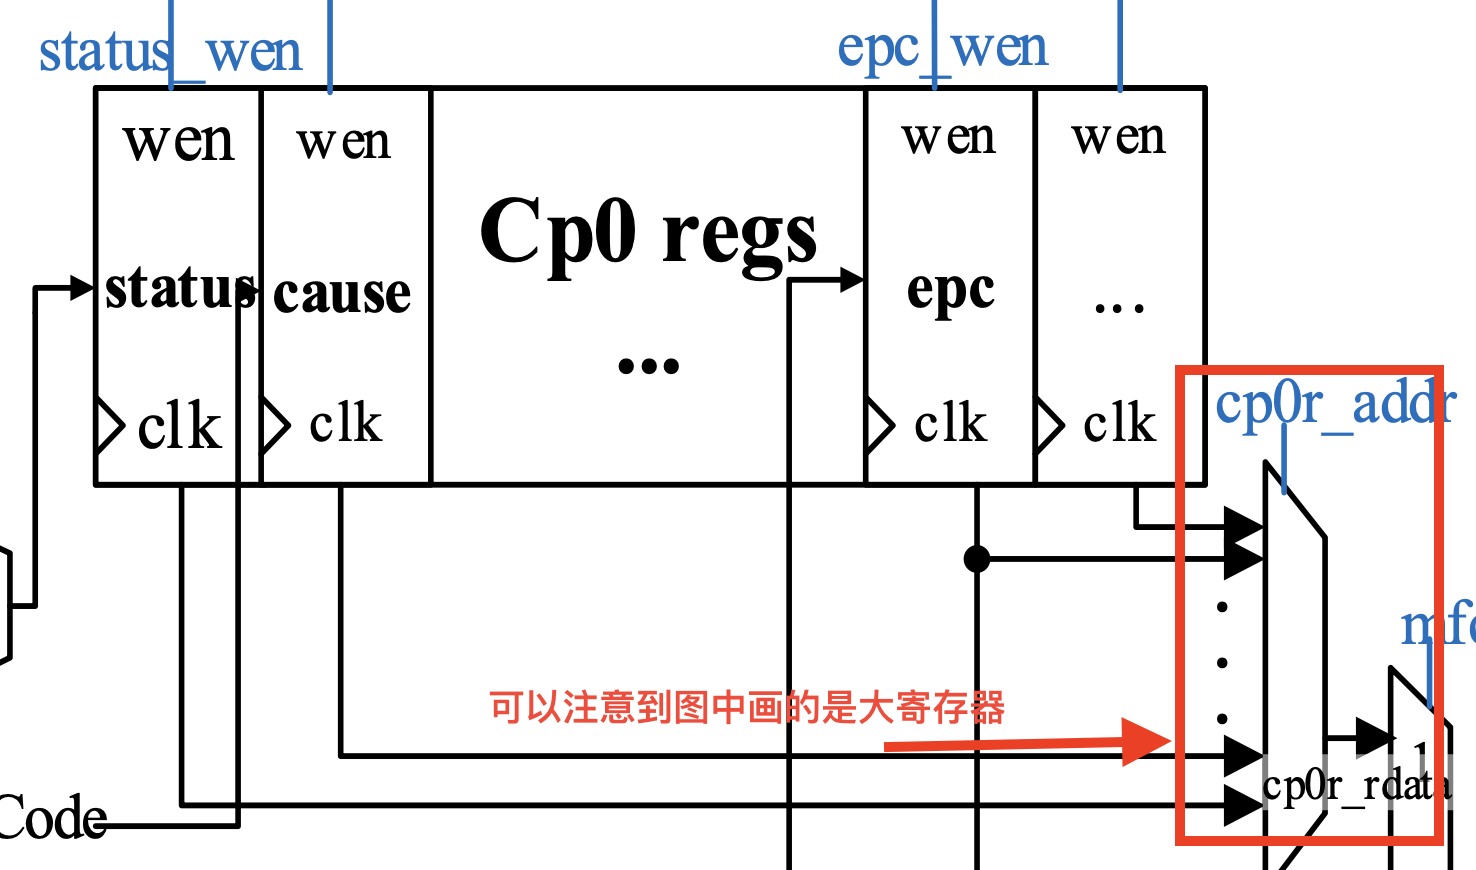
\includegraphics[width=0.6\textwidth]{img/复现流水线/cp0地址mux.png}
    \caption{CP0地址MUX}
\end{figure}


\paragraph{STATUS寄存器} STATUS寄存器是用于存放异常状态的寄存器,其中EXL(exception level)域是软件可读写的,故需要status\_wen信号。

要理解这个寄存器,重要的是知道syscall指令执行的时候发生了什么。因此,有必要单开一个小的章节来说明syscall指令执行的时候发生了什么。


\subsubsection{syscall指令执行流程}

SYSCALL指令在译码阶段被识别,并通过流水线总线传播到写回阶段:

\begin{lstlisting}[language=Verilog, caption=SYSCALL指令识别]
// 在decode.v中,SYSCALL指令的识别
assign inst_SYSCALL = (op == 6'b000000) & (funct == 6'b001100);
\end{lstlisting}

SYSCALL指令在五级流水线中的执行时序如下:

\begin{table}[H]
\centering
\caption{SYSCALL指令流水线执行时序}
\begin{tabular}{|c|c|c|c|c|c|}
\hline
\textbf{周期} & \textbf{IF} & \textbf{ID} & \textbf{EXE} & \textbf{MEM} & \textbf{WB} \\
\hline
1 & SYSCALL & - & - & - & - \\
\hline
2 & 下一条指令 & SYSCALL & - & - & - \\
\hline
3 & 下一条指令 & 下一条指令 & SYSCALL & - & - \\
\hline
4 & 下一条指令 & 下一条指令 & 下一条指令 & SYSCALL & - \\
\hline
5 & 下一条指令 & 下一条指令 & 下一条指令 & 下一条指令 & SYSCALL \\
\hline
6 & 异常处理程序 & 下一条指令 & 下一条指令 & 下一条指令 & 下一条指令 \\
\hline
\end{tabular}
\end{table}

当SYSCALL指令到达写回阶段时,执行以下关键操作:

\begin{lstlisting}[language=Verilog, caption=STATUS寄存器EXL域设置]
    always @(posedge clk)
    begin
        if (!resetn || eret)
        begin
            status_exl_r <= 1'b0;
        end
        else if (syscall)  // 如果遇到syscall指令,则将EXL域设置为1
        begin
            status_exl_r <= 1'b1;
        end
        else if (status_wen)
        begin
            status_exl_r <= mem_result[1];
        end
    end
    \end{lstlisting}

同时间,更新CAUSE寄存器:

\begin{lstlisting}[language=Verilog, caption=CAUSE寄存器异常编码设置]
    always @(posedge clk)
    begin
        if (syscall)
        begin
            cause_exc_code_r <= 5'd8;  // SYSCALL的异常编码为8
        end
    end
    \end{lstlisting}

这个寄存器用于存储发生异常的原因,这里设置为8,即SYSCALL的异常编码。


同时更新EPC寄存器:

\begin{lstlisting}[language=Verilog, caption=EPC寄存器保存当前PC]
    always @(posedge clk)
    begin
        if (syscall)
        begin
            epc_r <= pc;  // 保存产生异常的PC值
        end
        else if (epc_wen)
        begin
            epc_r <= mem_result;
        end
    end
    \end{lstlisting}

EPC是Exception Program Counter的缩写,用于存储产生异常的PC值。

同时,发出cancel信号:

\begin{lstlisting}[language=Verilog, caption=cancel信号发出]
    assign cancel = (syscall | eret) & WB_over;
\end{lstlisting}

这里有个名词叫做流水线的冲刷。同事补充一下异常入口跳转操作:
\begin{lstlisting}[language=Verilog, caption=异常PC总线]
    wire        exc_valid;
    wire [31:0] exc_pc;
    assign exc_valid = (syscall | eret) & WB_valid;
    assign exc_pc = syscall ? `EXC_ENTER_ADDR : cp0r_epc;
    assign exc_bus = {exc_valid, exc_pc}; // 分别代表异常有效和EPC寄存器的值
    \end{lstlisting}

总结一下SYSCALL指令执行流程:
    \begin{enumerate}
        \item \textbf{周期1-4}:SYSCALL指令在流水线中正常传播
        \item \textbf{周期5}:SYSCALL指令到达写回阶段,执行以下操作:
        \begin{itemize}
            \item STATUS[1] = 1(设置EXL域)
            \item CAUSE[6:2] = 8(设置异常编码)
            \item EPC = 当前PC(保存返回地址)
            \item cancel = 1(冲刷流水线)
            \item exc\_bus = \{1, 0\}(跳转到地址0)
        \end{itemize}
        \item \textbf{周期6}:IF跳转到地址0,开始执行异常处理程序
    \end{enumerate}

和所有的关键寄存器的变化过程:

\begin{table}[H]
    \centering
    \caption{SYSCALL执行前后关键寄存器状态}
    \begin{tabular}{|c|c|c|}
    \hline
    \textbf{寄存器} & \textbf{执行前} & \textbf{执行后} \\
    \hline
    STATUS[1] (EXL) & 0 & 1 \\
    \hline
    CAUSE[6:2] (ExcCode) & 0 & 8 \\
    \hline
    EPC & 任意值 & 产生异常的PC \\
    \hline
    PC & 产生异常的PC & 0(异常处理入口) \\
    \hline
    \end{tabular}
    \end{table}

\subsubsection{延迟槽机制实现的理解}

延迟槽机制在我看来就是编译器对指令排列优化后,然后CPU不用在对分支/跳转指令进行延时(stall)。最开始我是从Vivado的仿真中看出来这里有问题的:

\begin{figure}[H]
    \centering
    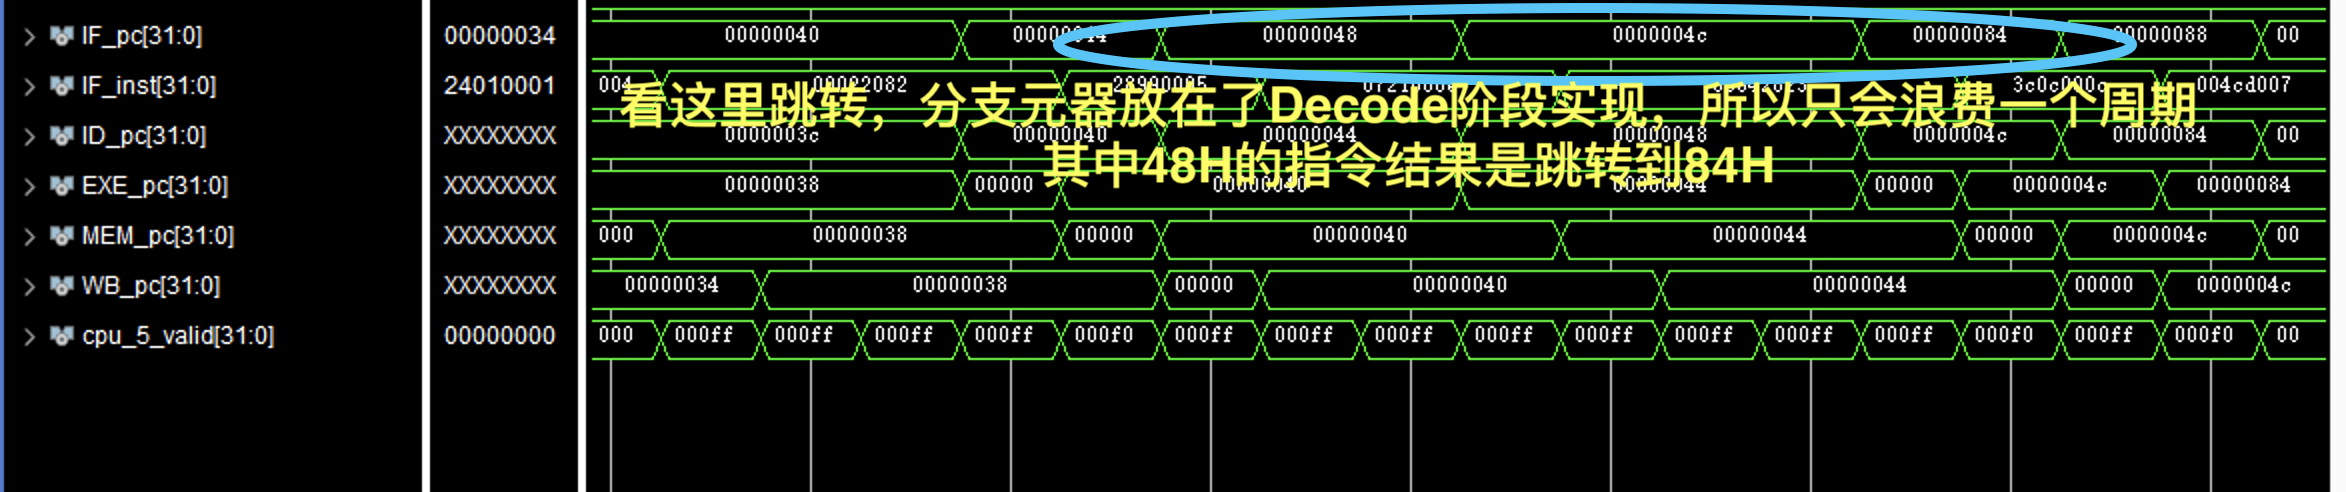
\includegraphics[width=\textwidth]{img/复现流水线/跳转1.png}
    \caption{延迟槽导致提前执行4CH指令}
\end{figure}

但是经过我观察指令集的排布,我感觉这里并不是错误,这里本身是48H指令(其结果是跳转到84H),那我们看一下到到底跳转过去要干嘛:


\begin{figure}[H]
    \centering
    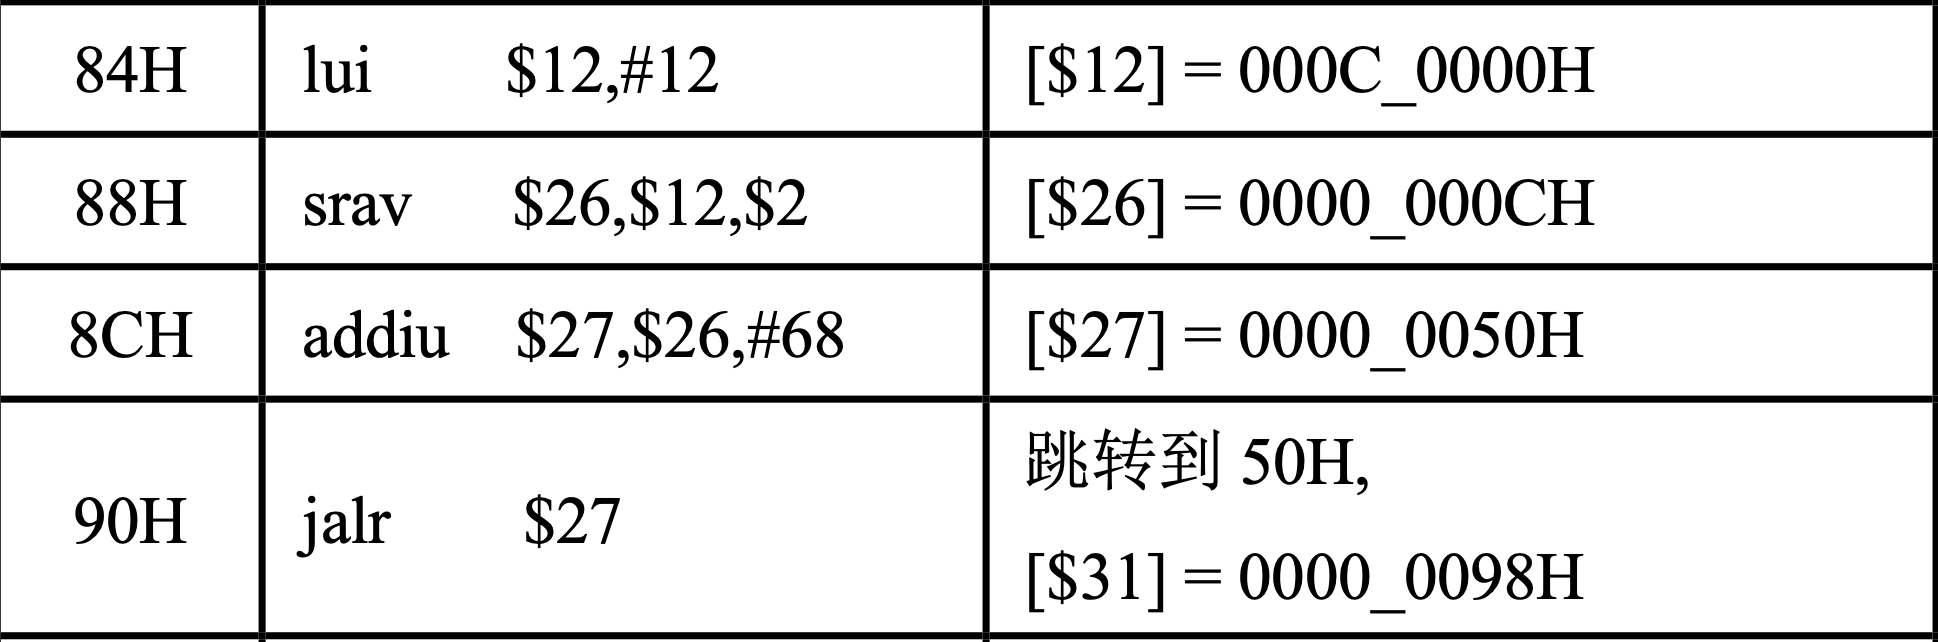
\includegraphics[width=0.75\textwidth]{img/复现流水线/84H.png}
    \caption{84H指令后续}
\end{figure}

可以看到他马上又跳转到到50H了,那么50H是在干嘛:

\begin{lstlisting}[language=Verilog]
    50H sw $5, #20($0) // 将$5寄存器的值存储到地址20处
\end{lstlisting}

回到这里的关键是多了一条4CH指令:


\begin{figure}[H]
    \centering
    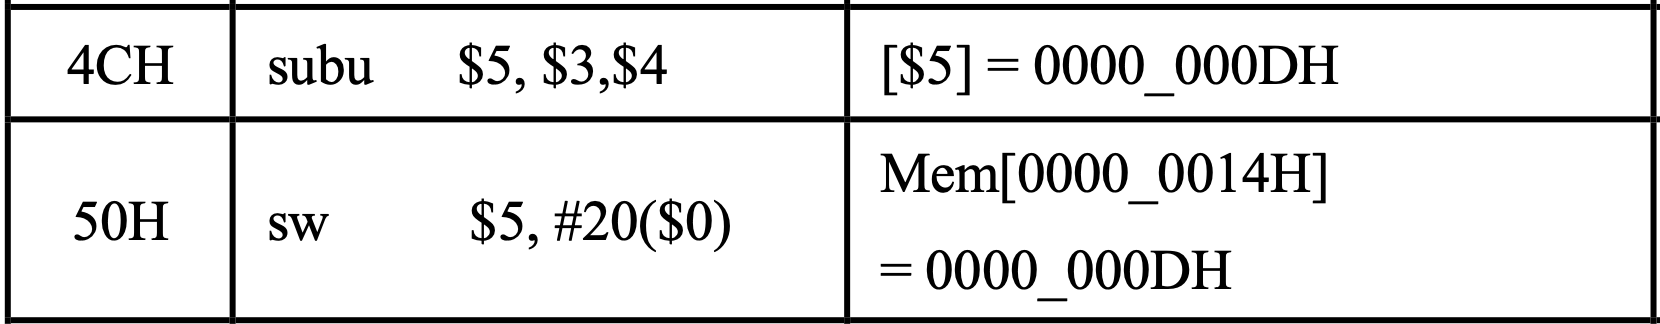
\includegraphics[width=0.75\textwidth]{img/复现流水线/4CH.png}
    \caption{4CH指令}
\end{figure}

可以看到指令的解释,也就是第三列,这个手册对50H指令的解释是:把0000\_000DH存储到5号寄存器中,而0000\_000DH这个值是怎么来的呢?答案是从4CH减过来的。因此这么执行我并不认为是错误的。

上学期我在写报告的时候,我还不太懂延迟槽机制,因此我认为这里是错误的,增加了一个stall。但是现在我认为我当时的修改是错误的。我认为这个CPU的整体工作状态是正确的。

\newpage

\subsection{配置IP核}

最后CPU的bug应该只有一个,就是如果使用原始的IP核,那么会让CPU多停滞一个周期,但是over等信号并没有因为多增加的寄存器而改变,所以我们这里只需要正确配置IP即可,同时,由于我没看懂源代码的IP是怎么弄的,我自己写了一个。


\begin{lstlisting}[language=Verilog]
    module inst_rom(
        clka,
        addra,
        douta
    );

    // ENTITY inst_rom_ip IS 这里是赛灵思的IP接口说明
    //   PORT (
    //     clka : IN STD_LOGIC;
    //     addra : IN STD_LOGIC_VECTOR(7 DOWNTO 0);
    //     douta : OUT STD_LOGIC_VECTOR(31 DOWNTO 0)
    //   );
    // END inst_rom_ip;

    input clka;
    input [7 : 0] addra;
    output [31 : 0] douta;

    inst_rom_ip entity (
    .clka(clka),
    .addra(addra),
    .douta(douta)
    );

    endmodule
\end{lstlisting}

其实我把赛灵思的IP接口说明拷贝过来注释就已经没有必要贴图片了,因为这个代码就是对xci文件/IP 核具体的描述,但是我这里还是贴上图片吧:

\begin{figure}[H]
    \centering    
    \begin{minipage}[t]{0.48\textwidth}
        \centering
        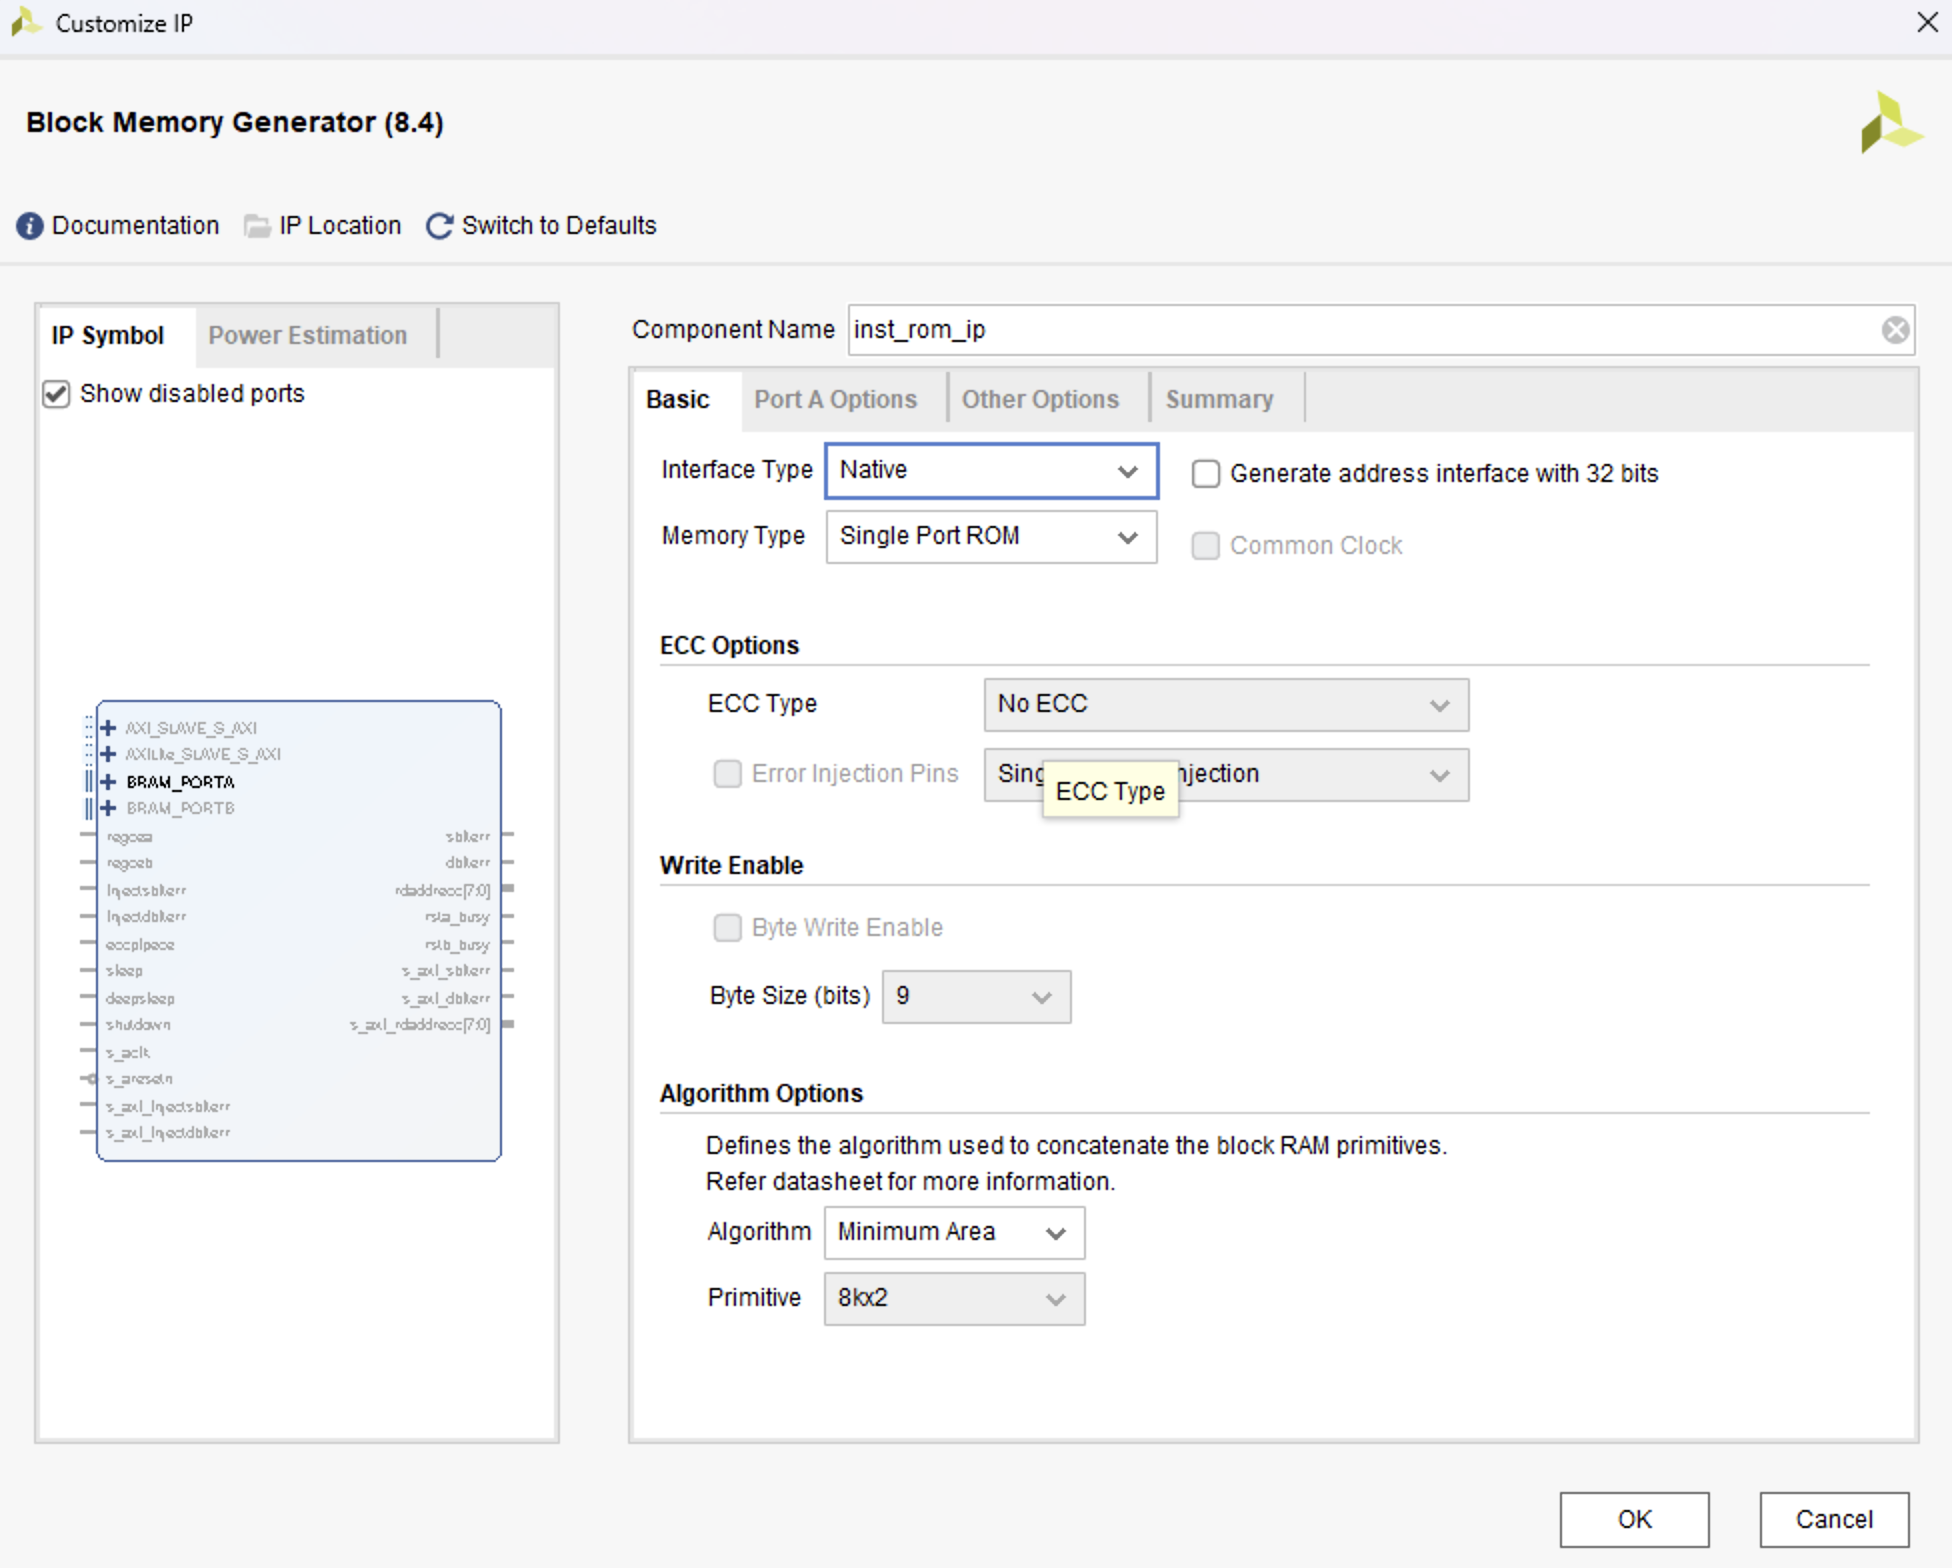
\includegraphics[width=\textwidth]{img/复现流水线/配置rom.png}
        \caption{rom选择}
    \end{minipage}
    \hfill
    \begin{minipage}[t]{0.48\textwidth}
        \centering
        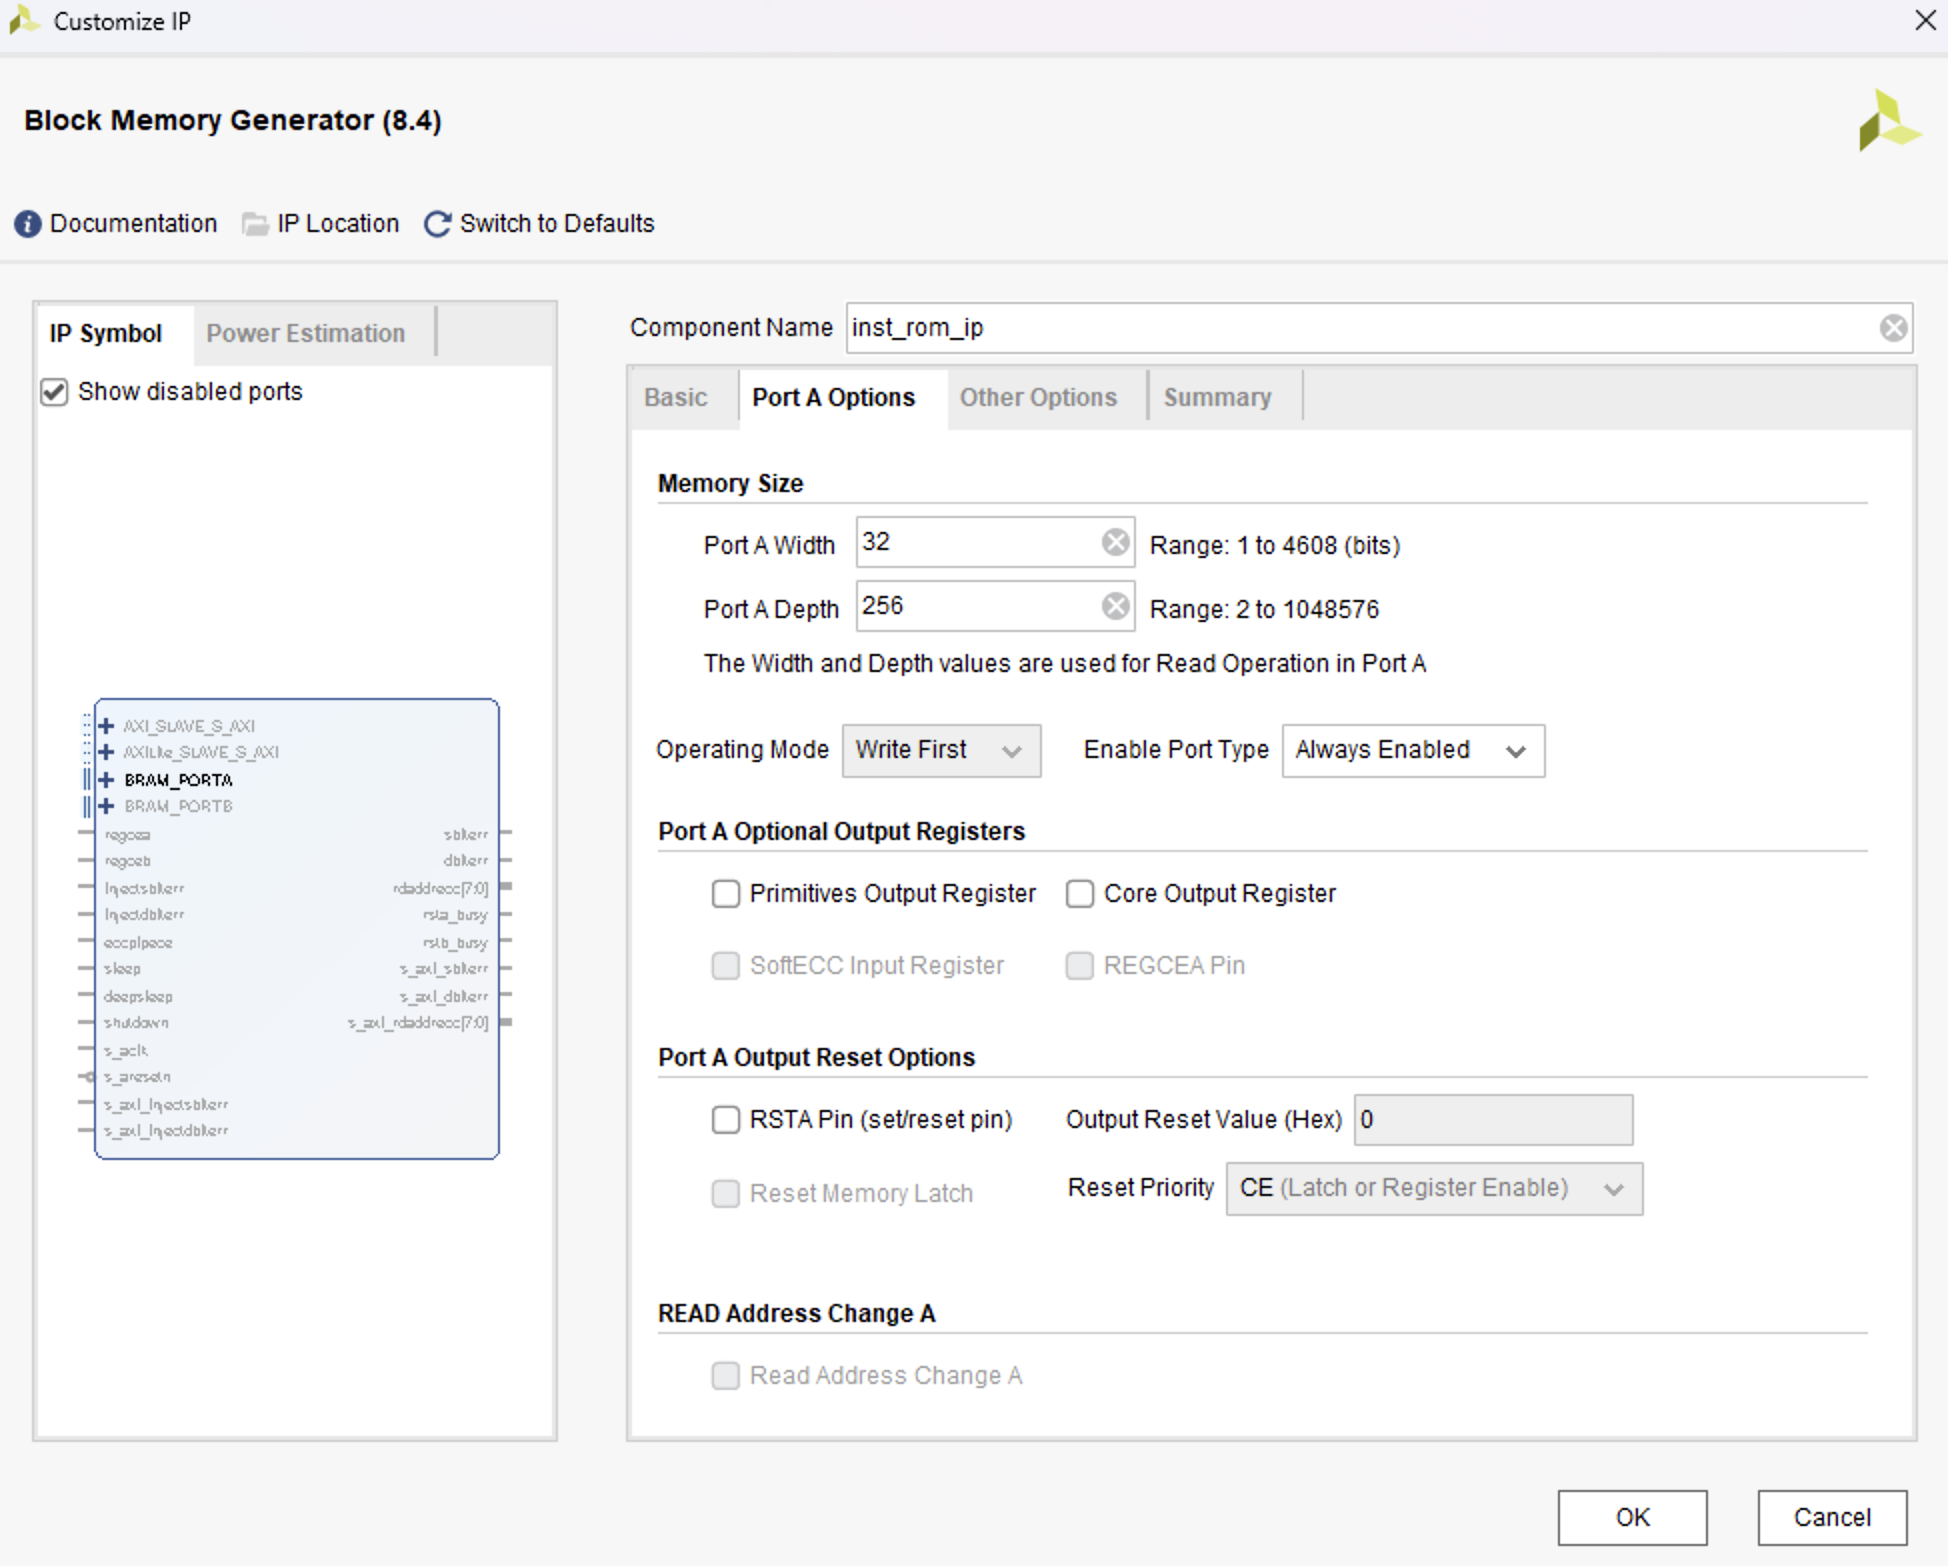
\includegraphics[width=\textwidth]{img/复现流水线/配置ram.png}
        \caption{rom配置}
    \end{minipage}
\end{figure}

同理于RAM,只是设置成了真双口。不过我看到网上有些对RAM的配置还选择了No-change模式,但是我的版本的vivado只有Write-first模式和Read-First。对于这里我还是不太懂,但是其他的设置是什么意思我比较清楚。


这里还可以说一下ROM的特点,就是这个代码写(或者说同步ROM导致)的导致他会等一个周期才能拿到指令:

\begin{figure}[H]
    \centering
    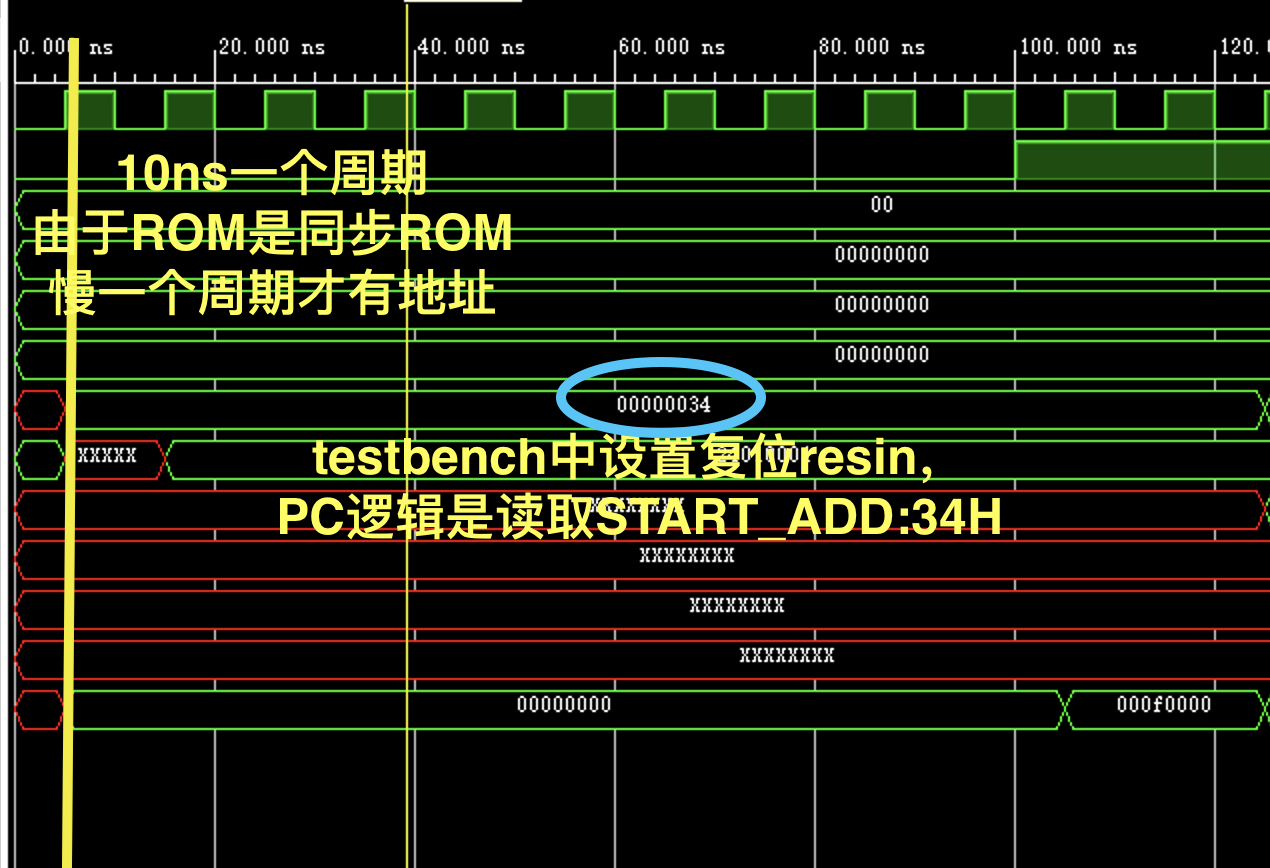
\includegraphics[width=0.75\textwidth]{img/复现流水线/刚进入.png}
    \caption{ROM特点}
\end{figure}

\newpage

\section{新增指令说明}


新增的指令有9条,分别如下表所示:

\begin{table}[H]
    \centering
    \begin{tabular}{ccc}
        \toprule
        序号 & 指令名称 & 汇编指令 \\
        \midrule
        1 & 有符号乘法 & mult rs, rt \\
        2 & 从LO寄存器取值 & mflo rd \\
        3 & 从HI寄存器取值 & mfhi rd \\
        4 & 向LO寄存器存值 & mtlo rs \\
        5 & 向HI寄存器存值 & mthi rs \\
        6 & 从cp0寄存器取值 & mfc0 rt, cs \\
        7 & 向cp0寄存器存值 & mtc0 rt, cd \\
        8 & 系统调用 & syscall \\
        9 & 异常返回 & eret \\
        \bottomrule
    \end{tabular}
    \caption{新增指令列表}
\end{table}

其中,syscall、mt/mfc0的作用在刚才为了讲解CP0寄存器的作用中已经讲过了,等下我他们直接分析在仿真中的行为。eret指令刚才没有说,但是它是用于异常返回的,也就是eret指令执行后,会跳转到EPC寄存器的值。换句话说,他总是和syscall指令成对出现的。

我们可以看到在coe文件中,30H的位置,也就是Exception Handler的结束位置,就是eret指令,他的作用是恢复现场,因此等下我也直接分析其仿真行为:

\begin{figure}[H]
    \centering
    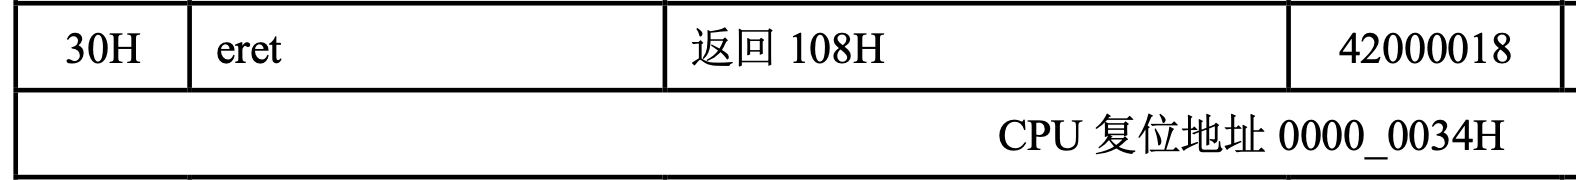
\includegraphics[width=0.75\textwidth]{img/复现流水线/handlerFinal.png}
    \caption{Exception Handler结束位置}
\end{figure}


\subsection{乘法器指令讲解}

乘法就是普通的乘法器实现的,没有做太多的优化。这里主要是关注HI和LO寄存器:

\begin{lstlisting}[language=Verilog, caption=乘法结果分配]
    //要写入HI的值放在exe_result里,包括MULT和MTHI指令
    //要写入LO的值放在lo_result里,包括MULT和MTLO指令
    assign exe_result = mthi     ? alu_operand1 :
                        mtc0     ? alu_operand2 : 
                        multiply ? product[63:32] : alu_result;
    assign lo_result  = mtlo ? alu_operand1 : product[31:0];
    assign hi_write   = multiply | mthi;
    assign lo_write   = multiply | mtlo;
    \end{lstlisting}

    可以看到,当出现multiply 指令或者mthi/mtlo指令的时候,EXE向下面的总线会包装上hi\_write/lo\_write信号,然后WB阶段会根据这个信号来写入HI/LO寄存器。

    \begin{table}[H]
        \centering
        \caption{乘法相关指令}
        \begin{tabular}{|c|c|c|}
        \hline
        \textbf{指令} & \textbf{功能} & \textbf{描述} \\
        \hline
        MULT rs, rt & 乘法运算 & 将rs×rt的结果存入HI/LO \\
        \hline
        MFHI rd & 从HI读取 & 将HI寄存器的值读入rd \\
        \hline
        MFLO rd & 从LO读取 & 将LO寄存器的值读入rd \\
        \hline
        MTHI rs & 向HI写入 & 将rs的值写入HI寄存器 \\
        \hline
        MTLO rs & 向LO写入 & 将rs的值写入LO寄存器 \\
        \hline
        \end{tabular}
    \end{table}

总结就是上面这个表格,那么具体地,我列出五个阶段的具体行为,等下仿真的时候我们验证:

\begin{enumerate}
    \item \textbf{译码阶段}:识别MULT指令,设置multiply信号
    \item \textbf{执行阶段}:
    \begin{itemize}
        \item 启动乘法器,开始多周期运算
        \item 等待mult\_end信号,表示乘法完成
        \item 将64位结果分为高32位和低32位
    \end{itemize}
    \item \textbf{访存阶段}:传递HI/LO写使能信号
    \item \textbf{写回阶段}:
    \begin{itemize}
        \item 将高32位写入HI寄存器
        \item 将低32位写入LO寄存器
    \end{itemize}
\end{enumerate}

\subsection{仿真行为}

\subsubsection{syscall与eret指令仿真行为}
首先我们分析sys和eret指令的仿真行为:

\begin{figure}[H]
    \centering
    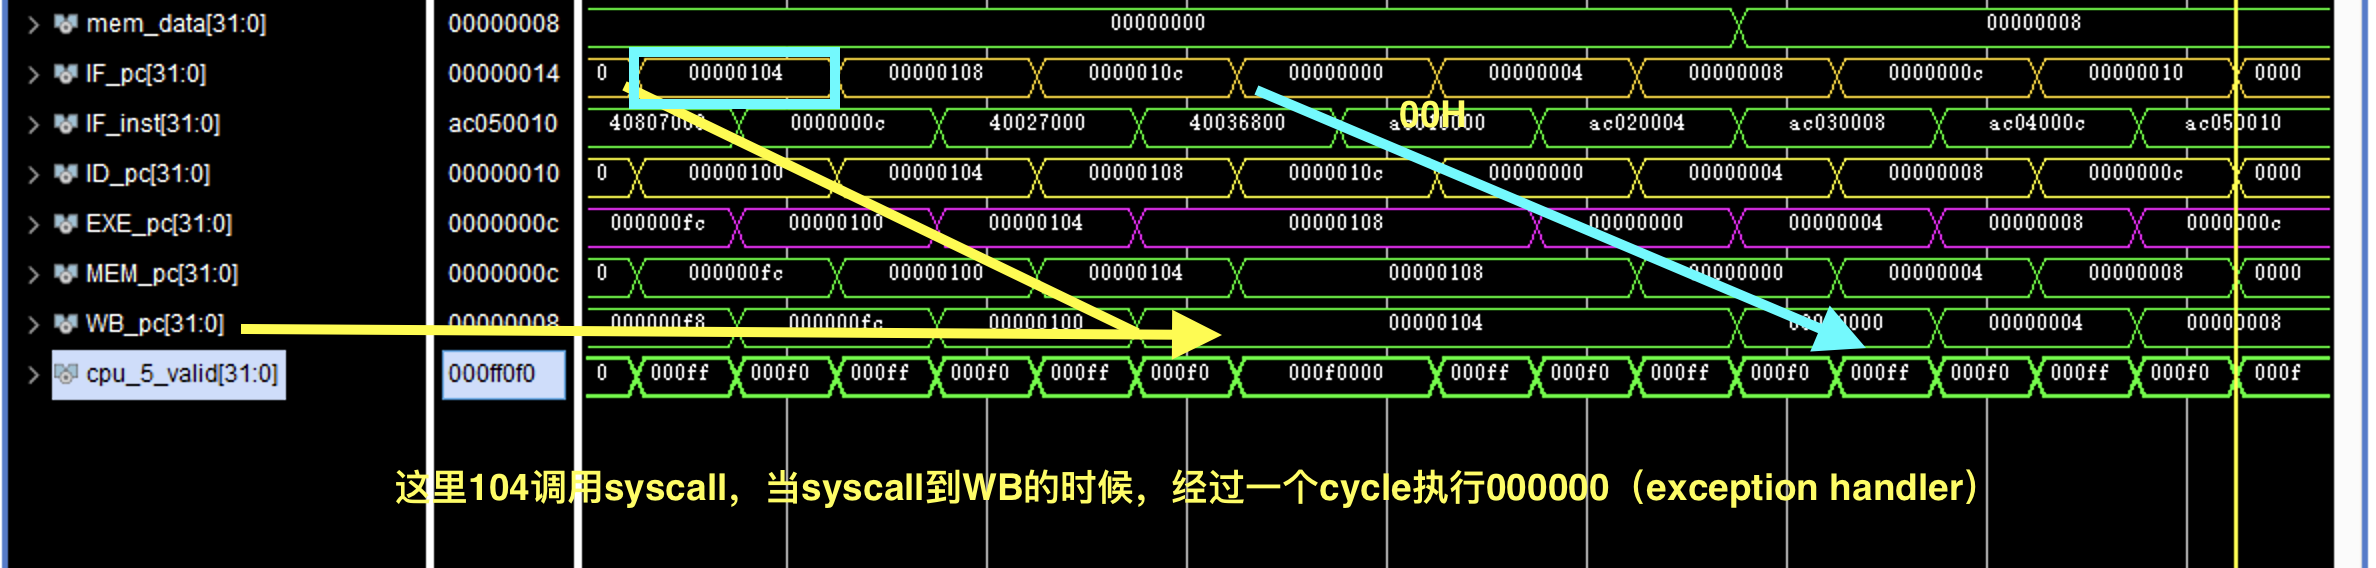
\includegraphics[width=\textwidth]{img/复现流水线仿真/syscall指令分析.png}
    \caption{syscall指令仿真行为}
\end{figure}

注意上面的执行,我挑选了104H这个位置(syscall的位置),之后由于syscall需要等到WB阶段才能执行,因此会多读出来两个指令(当到WB阶段的时,且需要经过一周期后,00H这个Handler才会进入到IF阶段,这个可以从设计图纸中看出,仿真图只是验证了其行为。

这里有必要插叙一个cancle信号:


\begin{lstlisting}[language=Verilog, caption=cancel信号]
    assign cancel = (syscall | eret) & WB_over;
\end{lstlisting}

这个信号是用于冲刷流水线的,也就是当syscall或eret指令执行完成后,会发出cancel信号,然后流水线会冲刷掉当前正在执行的指令,然后跳转到异常处理程序。


同时,在pipeline\_cpu.v中,IF允许进入的条件中也有cancel信号:

\begin{lstlisting}[language=Verilog, caption=cancel信号]
    assign IF_allow_in = (IF_over & ID_allow_in) | cancel;
\end{lstlisting}

这里时为了让IF可以立刻处理syscall的新指令,这点在syscall的仿真行为也得到验证,还是指刚过一周期的时候,假如108H或者10CH是乘法这种需要很多周期的指令,这个cancle信号依然能够保证IF可以立刻处理syscall的Exception Handler。


\begin{figure}[H]
    \centering
    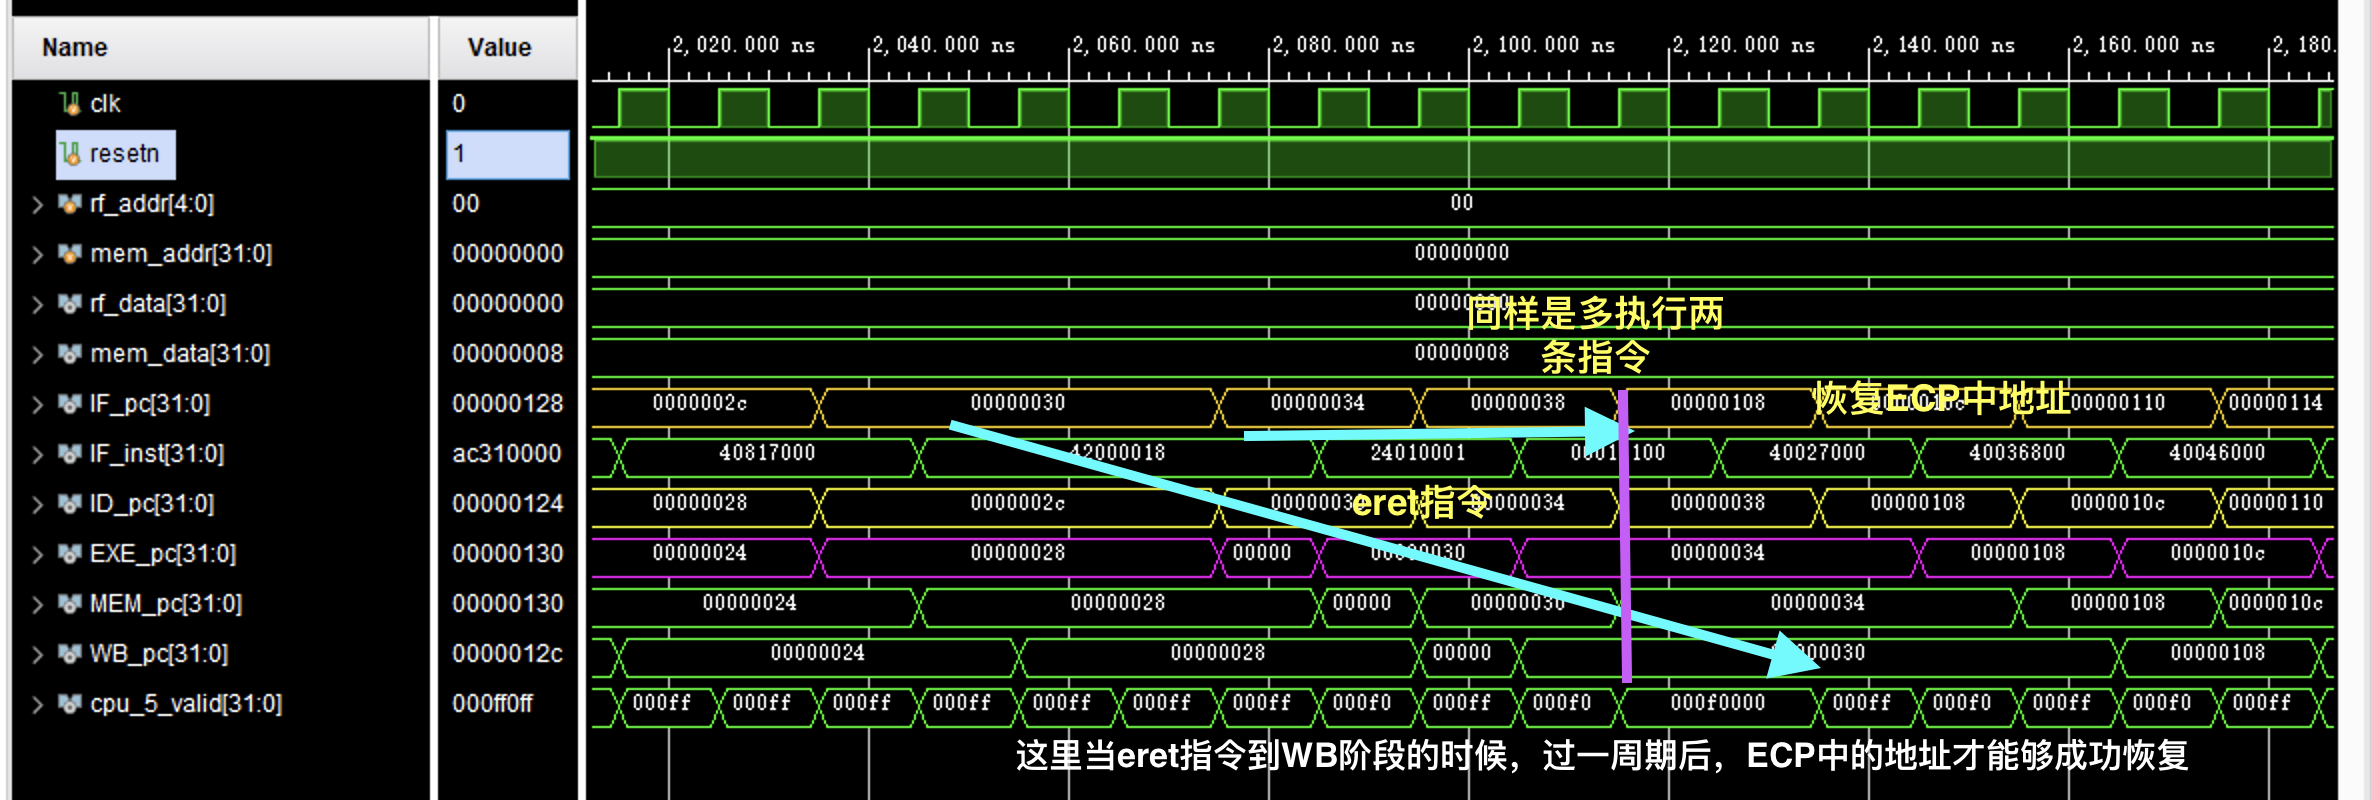
\includegraphics[width=\textwidth]{img/复现流水线仿真/eret指令分析.png}
    \caption{eret指令仿真行为}
\end{figure}

上图是eret指令(在30H)位置,执行完后(也就是在WB经过一周期后),108H立即开始执行(因IF的allow\_in信号由于cancel为1)。验证了我们的分析。

注意,这里我突然想解释一下多拿出来的这两个指令为什么又重复执行了,这到底正不正确。我认为是正确的,因为上面的syscall取出来的两个指令在还没到WB阶段的时候就被cancle信号全给冲刷掉了,因此相当于没执行。所以这里eret要接着从108H开始执行才对,这样才能保证正确恢复现场。

\subsubsection{有符号乘法}

有符号乘法就是普通的乘法器实现的,没有做太多的优化。因此会消耗非常多的周期:

\begin{figure}[H]
    \centering
    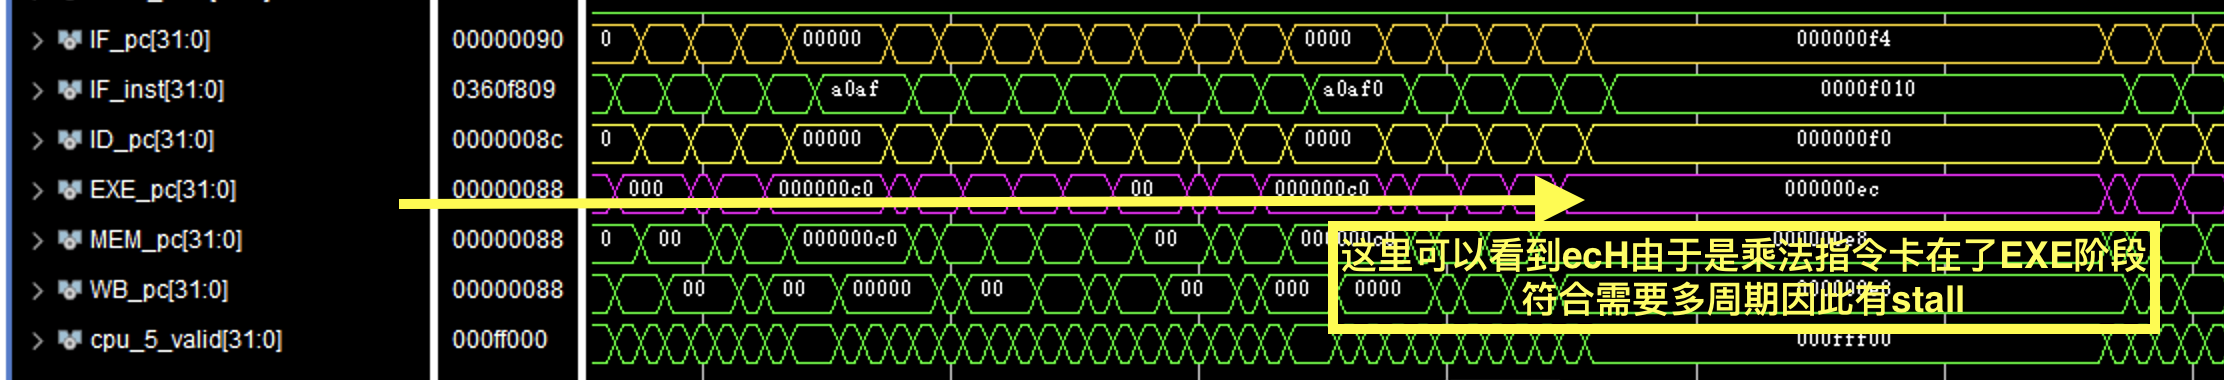
\includegraphics[width=\textwidth]{img/复现流水线仿真/多周期乘法卡在exe阶段.png}
    \caption{有符号乘法仿真行为}
\end{figure}

这里可以观察到ECH位置的乘法指令卡在了EXE阶段,因为多周期乘法器需要消耗非常多的周期。

由于仿真是看不出来具体的寄存器值的(我没有增加显示接口),所以我们这里通过分析顶层CPU提供的valid信号来分析:


\begin{figure}[H]
    \centering
    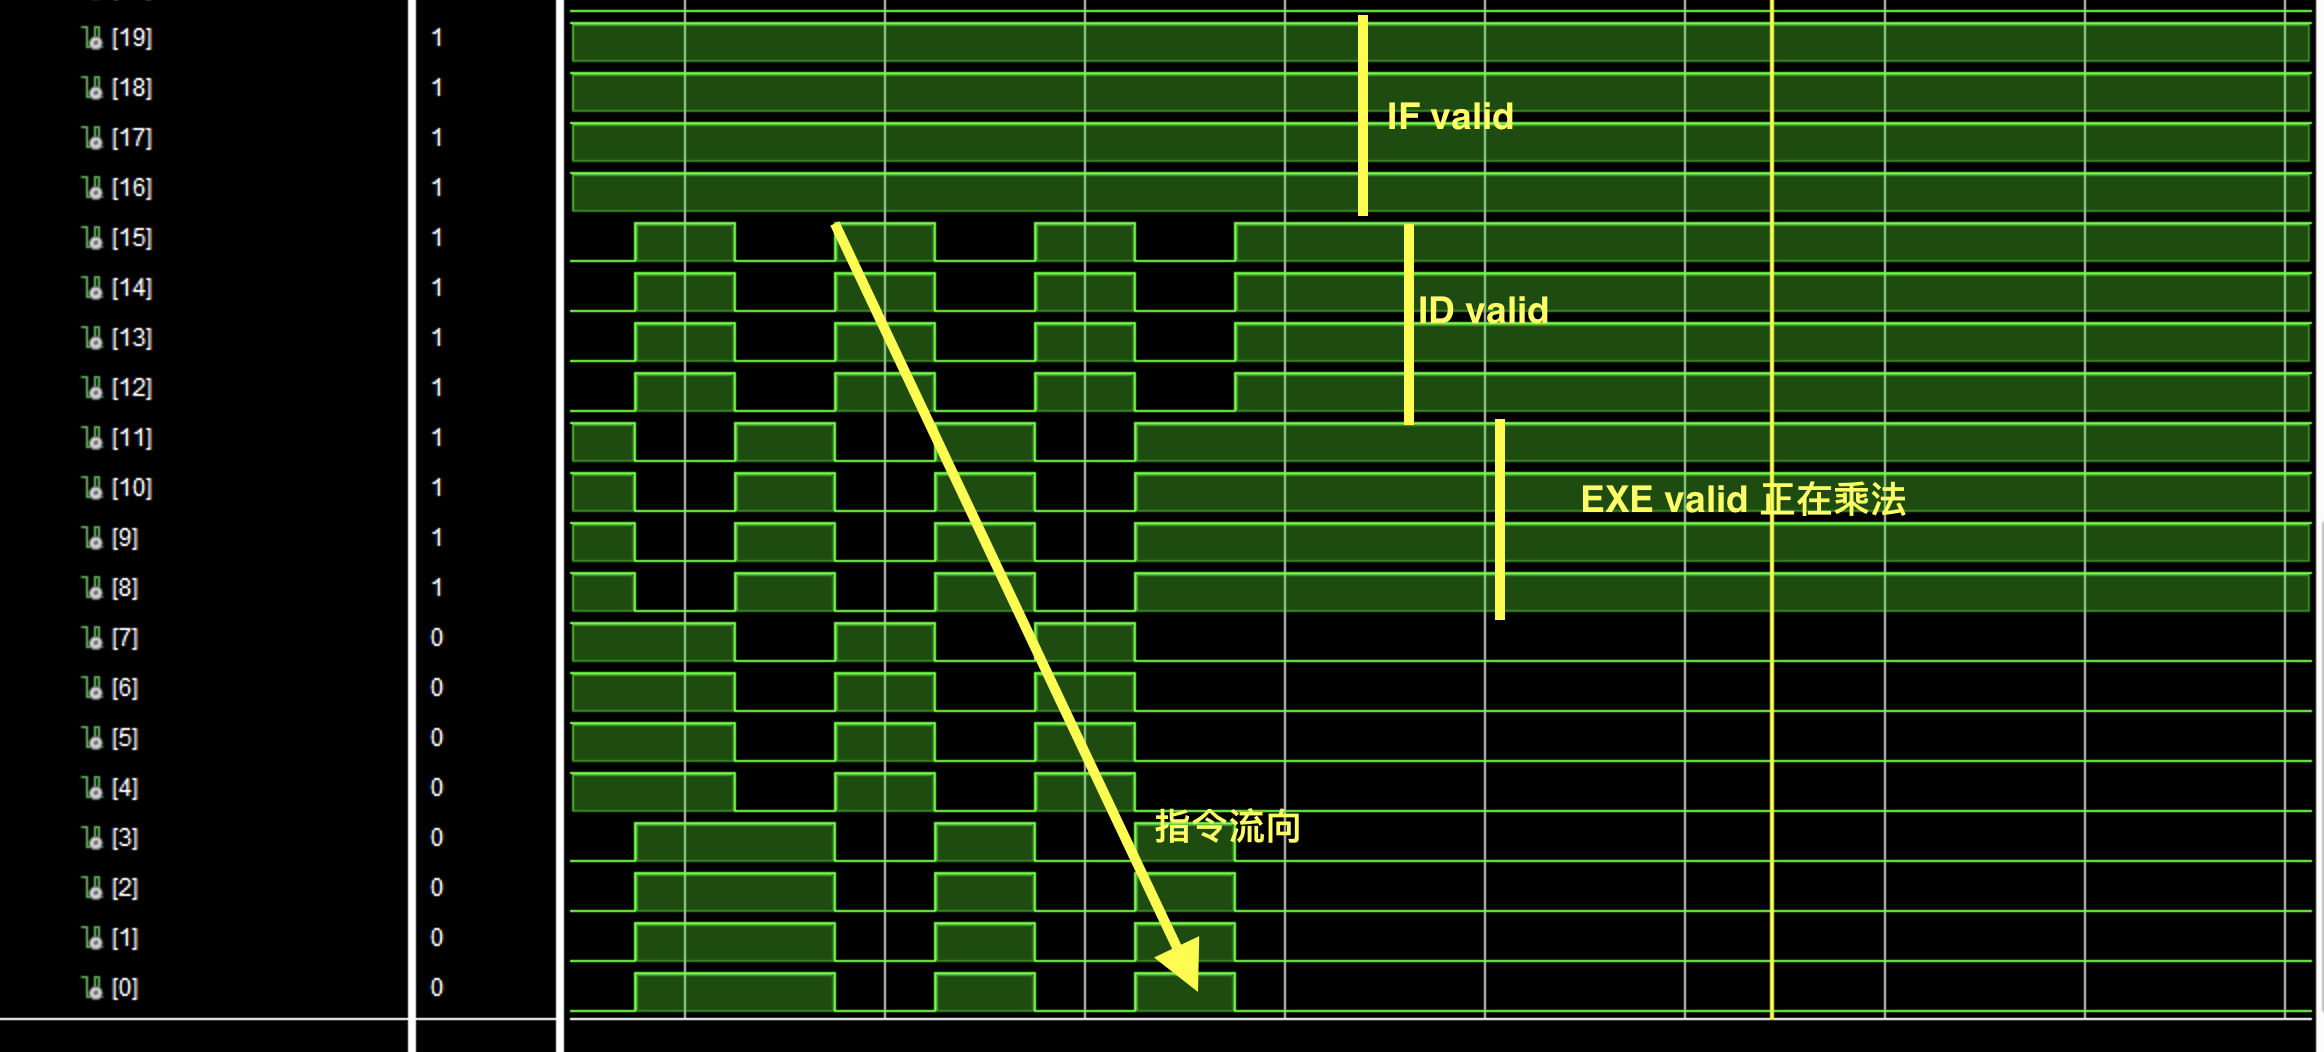
\includegraphics[width=0.75\textwidth]{img/复现流水线仿真/乘法valid行为.png}
    \caption{有符号乘法valid行为1}

    \centering
    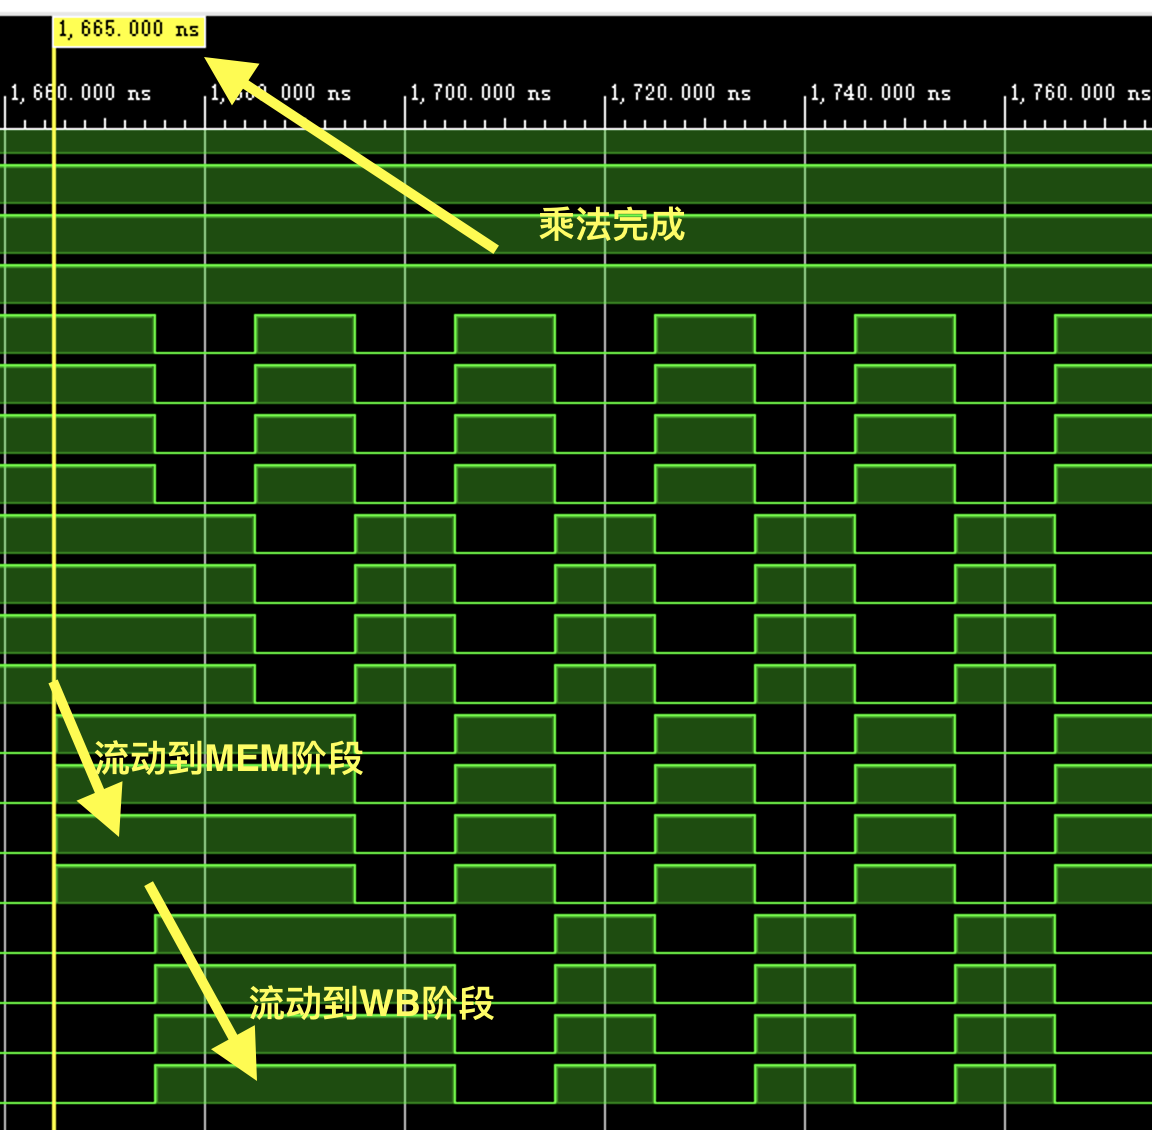
\includegraphics[width=0.75\textwidth]{img/复现流水线仿真/乘法完成后.png}
    \caption{有符号乘法valid行为2}
\end{figure}

通过分析他们的valid信号,就可以更详细的查看乘法的行为。大概情况就是valid从卡住,后面阶段的valid过两个周期后都为0了(数据为空),代表流水线停滞,等乘法完成后,后面阶段的valid又过两个周期后都为1了(数据有效),代表流水线继续执行。

\subsubsection{mfc0与mtc0指令仿真行为}

\begin{lstlisting}[language=Verilog]
    108H mfc0 $2, cp0(14.0)
    10CH mfc0 $3, cp0 (13.0)
    110H mfco $4, cp0 (12.0)
\end{lstlisting}

这三个指令是把cp0寄存器读取出来,然后写入到寄存器堆中。仿真图为:

\begin{figure}[H]
    \centering
    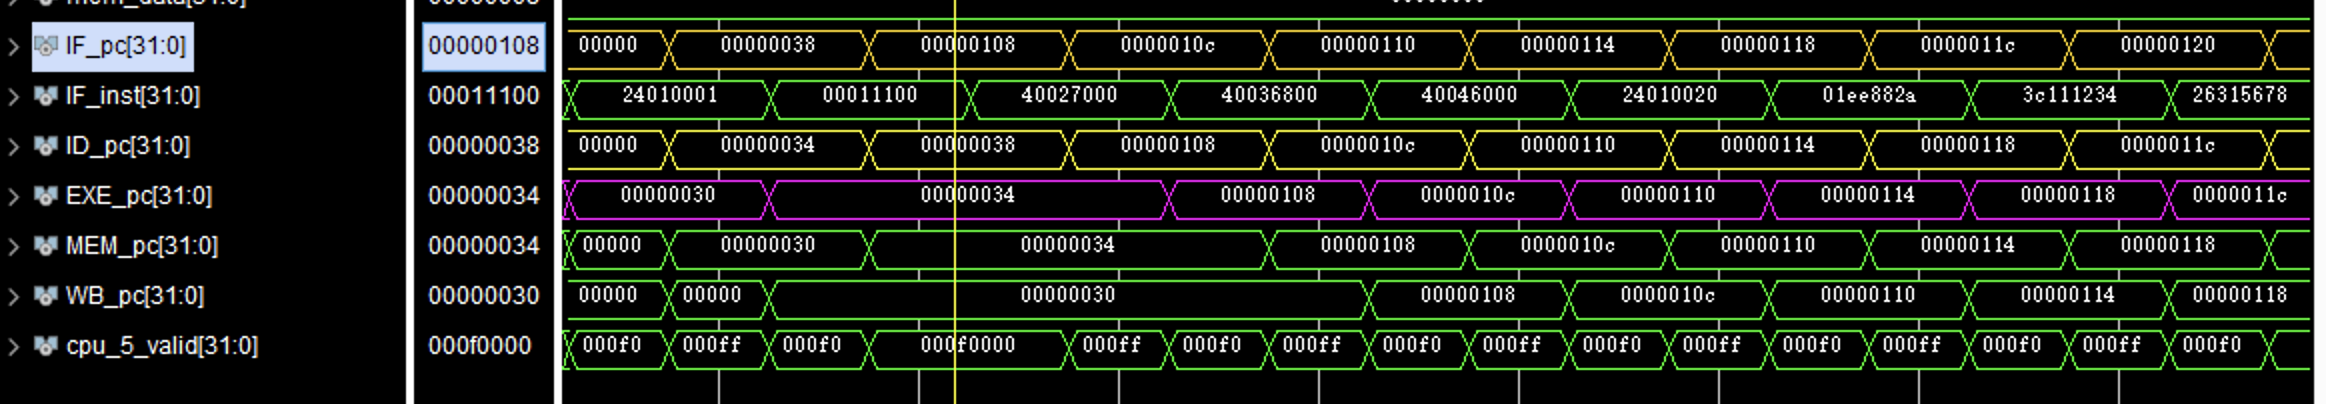
\includegraphics[width=\textwidth]{img/复现流水线仿真/mf.png}
    \caption{mfc0与mtc0指令仿真行为}
\end{figure}

由于仿真确实不太能看到详细结果,除非手动再引出一些显示接口。这里我们给出一个逻辑上的分析,口述一下mfc0指令调用的时候发生了什么:

\paragraph{decode阶段} 

在decode.v中,MFC0指令的识别逻辑:

\begin{lstlisting}[language=Verilog, caption=MFC0指令识别]
assign inst_MFC0 = (op == 6'b010000) & (rs==5'd0) 
                & sa_zero & (funct[5:3] == 3'b000);
\end{lstlisting}

\textbf{译码条件}:
\begin{itemize}
    \item 操作码为010000(协处理器0指令)
    \item rs域为0(源寄存器为0)
    \item sa域为0(特殊域为0)
    \item funct[5:3]为000(协处理器0操作)
\end{itemize}

除此之外:

\begin{lstlisting}[language=Verilog, caption=ID阶段MFC0信号生成]
    assign mfc0 = inst_MFC0;
    assign cp0r_addr = {rd, cp0r_sel};  // rd=14, cp0r_sel=0
    \end{lstlisting}

    \textbf{关键信号}:
\begin{itemize}
    \item \texttt{mfc0 = 1}:标识为MFC0指令
    \item \texttt{cp0r\_addr = 14}:目标CP0寄存器地址
    \item \texttt{rf\_wen = 1}:需要写回寄存器堆
    \item \texttt{rf\_wdest = 2}:目标寄存器为\$2
\end{itemize}

\paragraph{execute阶段} 

在exe阶段:

\begin{lstlisting}[language=Verilog, caption=EXE阶段MFC0处理]
    // MFC0指令在EXE阶段不需要ALU运算
    // 直接传递控制信号到后续阶段
    assign EXE_MEM_bus = {..., mfc0, ..., rf_wen, rf_wdest, ...};
    \end{lstlisting}

    \textbf{执行特点}:
    \begin{itemize}
        \item 不需要ALU运算
        \item 直接传递控制信号
        \item 准备CP0寄存器读取
    \end{itemize}


    \paragraph{memory阶段} 
在MEM阶段主要涉及这些代码:

    \begin{lstlisting}[language=Verilog, caption=MEM阶段MFC0处理]
        // MEM阶段继续传递MFC0信号
        assign MEM_WB_bus = {..., mfc0, ..., rf_wen, rf_wdest, ...};
        \end{lstlisting}
        
        \textbf{处理过程}:
        \begin{itemize}
            \item 继续传递MFC0控制信号
            \item 准备CP0寄存器数据读取
            \item 维护寄存器写回信息
        \end{itemize}

        \paragraph{write back阶段} 
        最后WB阶段会读取CP0寄存器,然后写入到寄存器堆中:

        \begin{lstlisting}[language=Verilog, caption=WB阶段CP0寄存器读取]
            // CP0寄存器读取逻辑
            wire [31:0] cp0r_rdata;
            assign cp0r_rdata = (cp0r_addr=={5'd12,3'd0}) ? cp0r_status :
                               (cp0r_addr=={5'd13,3'd0}) ? cp0r_cause  :
                               (cp0r_addr=={5'd14,3'd0}) ? cp0r_epc : 32'd0;
            
            // 寄存器堆写回数据选择
            assign rf_wdata = mfhi ? hi :
                              mflo ? lo :
                              mfc0 ? cp0r_rdata : mem_result;
            \end{lstlisting}
            
            \textbf{关键操作}:
            \begin{itemize}
                \item 根据cp0r\_addr=14,读取EPC寄存器
                \item 将EPC寄存器的值作为rf\_wdata
                \item 写回到\$2寄存器
            \end{itemize}


到此为止,mfc0指令的行为就分析完了。

\section{实验总结}

\begin{enumerate}
    \item 我自行学习了级联控制,对延迟槽机制更加熟悉了。
    \item 详细分析了syscall、eret、mfc0、mtc0指令的行为,并给出了逻辑上的分析。
    \item 有一个地方最开始一直没看懂,就是为什么有些指令即使读进去也认为没问题(我指syscall的后面两条),后来想通了,我认为应该是由于这两条指令是没有机会走到WB阶段的,因此不会造成实质性影响。
    \item 总的来说我更加熟悉CPU了,我打算国庆的时候把这学期要求的功能能实现多少实现多少。
\end{enumerate}

\label{LastPage}

\end{document}